\chapter{Instance Radiosity}\label{chp:instant-radiosity}
\textit{Instant radiosity}\cite{a:InstantRadiosity}, which was introduces by Alexander Keller in 1997, is related to bidirectional path tracing (see section \ref{sec:bidirectional-path-tracing} in chapter \ref{chp:path-tracing}) and a two-pass methods. The eye paths are only one segment long. On the other hand, more than one light path is combined with each eye-path vertex. The same set of light paths is used for all eye paths.

Under the assumption of diffuse reflection, in the light path, this algorithm generates a particle approximation of the diffuse radiance in the scene using the quasi-random walk based on the method of quasi-Monte Carlo integration. 

Then, in the eye path, the graphics hardware renders an image with shadows for each particle used as point light source. Global illumination finally is obtained by summing up the single images in an accumulation buffer and displaying the result.

The main advantage of instant radiosity is in the so-called positively correlated sampling for all pixels. Because the same light paths are used for all pixels, images computed with instant radiosity look smoother and lack the typical noisy artifacts of (bidirectional) path tracing. In addition, the shadow rays traced between eye-path vertices and the light-path vertices are highly coherent (see section \ref{sec:coherent-ray-tracing} in chapter \ref{chp:path-tracing}), similar to eye rays traced in ray casting. They can be traced significantly faster than in (bidirectional) path tracing.

The main limitation of IR is that it typically can only be used with diffuse or moderately glossy surfaces, the reason being that only relatively few paths (several hundreds) are created and thus the set of all possible light paths is only sparsely sampled.




\section{The Basic Algorithm}
Our eyes perceive radiance, which is power per unit area per unit solid angle. In vacuum the radiance $L$ fulfills the radiance equation:

\begin{equation*}
\begin{aligned}
	L(y,\vec{\omega}_r)&=L_e(y,\vec{\omega}_r)+\int_\Omega f_r(\vec{\omega}_i,y,\vec{\omega}_r)L(h(y,\vec{\omega}_i),-\vec{\omega}_i)cos\theta_id\vec{\omega}_i\\
	&:=L_e+T_{f_r}L
\end{aligned}
\end{equation*}

Given the quadruple $(S,f_r,L_e,\Psi)$, the global illumination problem consists in calculating functionals of the form:

\begin{equation*}
	\langle L,\Psi\rangle :=\int_S\int_\Omega L(y,\vec{\omega})\Psi(y,\vec{\omega})cos\theta d\omega dy
\end{equation*}

either in the radiosity setting or for the full radiance equation. That is, we project the solution onto a set of basis vectors $(\Psi_k)^{K}_{k=1}$ by $\Phi_k=\langle L,\Psi_k\rangle$. So the radiance calculation can be written as:

\begin{equation}
\begin{aligned}
	\overline{L}_{mn}:=\langle L,\Psi_{mn}\rangle &=\langle L_e,\Psi_{mn}\rangle+\langle T_{f_r}L,\Psi_{mn} \rangle \\
	&=\langle L_e,\Psi_{mn} \rangle+T_{mn}L
\end{aligned}
\end{equation}

passing through a pixel $P_{mn}$, where the shorthand $T_{mn}L$ defines the rendering operator, which determines the at least once reflected radiance through $P_{mn}$. If the radiance $L$ in the radiosity setting can be approximated by a discrete density of $M$ point light sources:

\begin{equation}\label{e:m-point-light-approximation}
	L(y)\approx\sum^{M-1}_{i=0}L_i\delta(y-P_i)
\end{equation}

where $L_i$ is the radiance and $P_i$ is the position of the $i$-th light source, the application of $T_{mn}$ to the particle approximation yields the very fast rendering algorithm:

\begin{equation*}
	\overline{L}_{mn}\approx \langle L_e,\Psi_{mn}\rangle+\sum^{M-1}_{i=0}T_{mn}L_i\delta(y-P_i)
\end{equation*}

where $T_{mn}$ applied to a point light source simultaneously can be evaluated for all pixels of the image matrix by calling a standard graphics hardware illumination routine, producing the shaded image of the textured scene including shadows. So the main algorithm of IR is to generate a particle approximation of the diffuse in the scene.

The directly visible light source in $\langle L_e,\Psi_{mn}\rangle$ and all the indirect point light sources are rendered on the fly by assigning emission to the corresponding surface elements (see figure \ref{f:instant-radiosity}). The algorithm thus directly operates on the textured scene description in image space and does not apply any kernel or solution discretization to the integral equation.

A small number (usually 50...300) of point light sources will be sufficient, since from multipass rendering with expensive local pass calculations, it is known that a very coarse radiosity solution suffices to produce realistic images. So the speed of the algorithm mainly depends on the frame generation rate of the graphics hardware, promising interactive rates of photorealistic image generation.



\subsection{Quasi-Monte Carlo Integration}
It uses the method of quasi-Monte Carlo integration (see section \ref{sec:quasi-monte-carlo}) for the evaluation of the integrals due to its fast convergence. For the approximation:

\begin{equation*}
	\int_{[0,1)^{s}}f(x)dx\approx\frac{1}{N}\sum^{N-1}_{i=0}f(x_i)
\end{equation*}

it generates the $N$ sample points $x_0,\cdots ,x_{N-1}\in [0,1)^{s}$ using the Halton sequence\footnote{\url{https://en.wikipedia.org/wiki/Halton_sequence}}. It based on radical inversion, which transfers the natural number $i$ into base-$b$-representation and mirrors that representation at the decimal point, resulting in the radical inverse function:

\begin{equation*}
	\Phi_b(i):=\sum^{\infty}_{j=0}a_j(i)b^{-j-1}\Leftrightarrow i=\sum^{\infty}_{j=0}a_j(i)b^{j}
\end{equation*}


The $s$-dimensional Halton low discrepancy sequence is built by:

\begin{equation*}
	x_i=(\Phi_{b_1}(i),\cdots,\Phi_{b_s}(i))
\end{equation*}

where the base $b_j,1\leq j\leq s$, mostly is chosen to be the $j$-th prime number.




\subsection{The Quasi-Random Walk}
Taking the diffuse part of the scene, the operator norm can be estimated by the mean reflectivity:

\begin{equation*}
	\overline{\rho}:=\frac{\sum^{k}_{k=1}\rho_{d,k}|A_k|}{\sum^{k}_{k=1}|A_k|}\approx ||T_{f_d}||
\end{equation*}

where the scene $S:=\bigcup^{K}_{k=1}A_k$ is composed of $K$ surface elements $A_k$ with average diffuse reflectivity of $\rho_{d.k}$.

As in \cite{a:Quasi-MonteCarloRadiosity}, the radiosity density is simulated by its particle nature using the technique of the quasi-random walk. Since in realistic scene models the actual diffuse reflectivity has only small deviation from $\overline{\rho}$, we can use fractional absorption and avoid Russian Roulette absorption. So from $N$ particles started at the light sources, $\overline{\rho}N$ particles are supposed not to be absorbed by the first reflection, $\overline{\rho}^{2}N$ survive the second reflection and so on. Then the number $M$ of radiance points generated is bounded by:

\begin{equation*}
	M<\sum^{\infty}_{j=0}\overline{\rho}^{j}N=\frac{1}{1-\overline{\rho}}N=:\overline{l}N
\end{equation*}

and thus is linear in $N$ depending on the average scene reflectivity $\overline{\rho}$, where $\overline{l}$ is the mean path length. The quasi-random walk scheme now evaluates $T_{mn}L_e$ using $N$ point lights, $T_{mn}T_{f_d}L_e$ by using $\lfloor\overline{\rho}N\rfloor$ point lights, and so on, where the particles are generated using the Halton sequence. 



\subsection{Implementation}
The pseudocode of the instant radiosity algorithm is given in algorithm \ref{al:instant-radiosity}. To generate the discrete density approximation of $p_j$ by low discrepancy points, it first fixes the number $N$ of particles to start off the light source. By an isometry $y_0$ the first two components of the Halton sequenc are mapped from the unitsquare onto the surface of the light source, yielding the starting point $y=y_0(\Phi_2,\Phi_3)$ with power $L=L_e(y)$ supp $L_e$.

Exploiting the property of the Halton sequence that segments of the sequence have small discrepancy, too, $\lfloor\overline{\rho}N\rfloor$ first points are used to shoot a ray into direction $\vec{\omega}$ using:

\begin{equation*}
	\vec{\omega}=\vec{\omega}_d(\Phi_{b_{2j+2}},\Phi_{b_{2j+3}})=(arcsin\sqrt{\Phi_{b_{2j+2}}},2\pi\Phi_{b_{2j+3}})
\end{equation*}

where the direction already is distributed with respect to the cosine-term in density $p_j$. In the next hitpoint $y=h(y,\vec{\omega})$ the particle's radiance is attenuated by $f_d(y)$. From these particles the first $\lfloor\overline{\rho}^{2}N\rfloor$ continue their paths, repeating the diffuse scattering procedure until no particles remain.

\begin{algorithm}\label{al:instant-radiosity}
\begin{lstlisting}[language=C++,mathescape]
void InstantRadiosity(int $N$, double $\overline{\rho}$){
	double $\omega$,Start;
	int End,Reflections=0; 
	Color $L$; Point $y$; Vector $\vec{\omega}$;
	
	Start = End = $N$; 
	while(End > $0$){
		Start *= $\overline{\rho}$;
		for(int $i$ = (int) Start; $i$ < End; $i$++)
			// Select starting point on light source
			$y=y_0(\Phi_2(i),\Phi_3(i))$;
			$L=L_e(y)*$ supp $L_e$;
			$\omega=N$;
		
			// trace reflections
			for(int $j$ = 0; $j$ <= Reflections; $j$++)
				glRenderShadowedScene($\frac{N}{\lfloor\omega\rfloor}L,y$); 
				glAccum(GL_ACCUM, $\frac{1}{N}$);
				// diffuse scattering
				$\vec{\omega}=\vec{\omega}_d(\Phi_{b_{2j+2}}(i),\Phi_{b_{2j+3}}(i))$;
				//trace ray from $y$ into direction $\vec{\omega}$
				$y=h(y,\vec{\omega})$;
				// Attenuate and compensate
				$L*=f_d(y)$;
				$\omega *=\vec{\rho}$;
			}
		}
    
		Reflections++;
		End = (int) Start;
	}
	
	glAccum(GL RETURN, 1.0);
}                                                                                
\end{lstlisting}	
\caption{Instant radiosity pseudocode}
\end{algorithm}

The starting points and the subsequent hitpoints of the above quasi-random walk then form the discrete density approximation \ref{e:m-point-light-approximation} which is used for the hardware lighting call glRenderShadowedScene, i.e, the scene is rendered with shadows and the point light source licated in $y$ with the power $\frac{N}{\lfloor\omega\rfloor}L$. Finally the quasi-Monte Carlo integration is performed by accumulating all images with the weight $\frac{1}{N}$.

The algorithm displayed in algorithm \ref{al:instant-radiosity} is illustrated by figure \ref{f:instant-radiosity}. For a path number of $N=10$ the single images created by the point light sources (red balls) are shown. Point light sources are placed at the locations where these trajectories hit object surfaces. The direct illumination due to these point light sources (Images 1 to 20) is accumulated. Image A shows the result of accumulating the Images 1 to 10, with light source points at the origin of the simulated trajectories, on the extended light source. This results in direct illumination due to the extended light source.

\begin{figure*}\label{f:instant-radiosity}
\begin{center}
	\begin{subfigure}[b]{0.38\textwidth}
		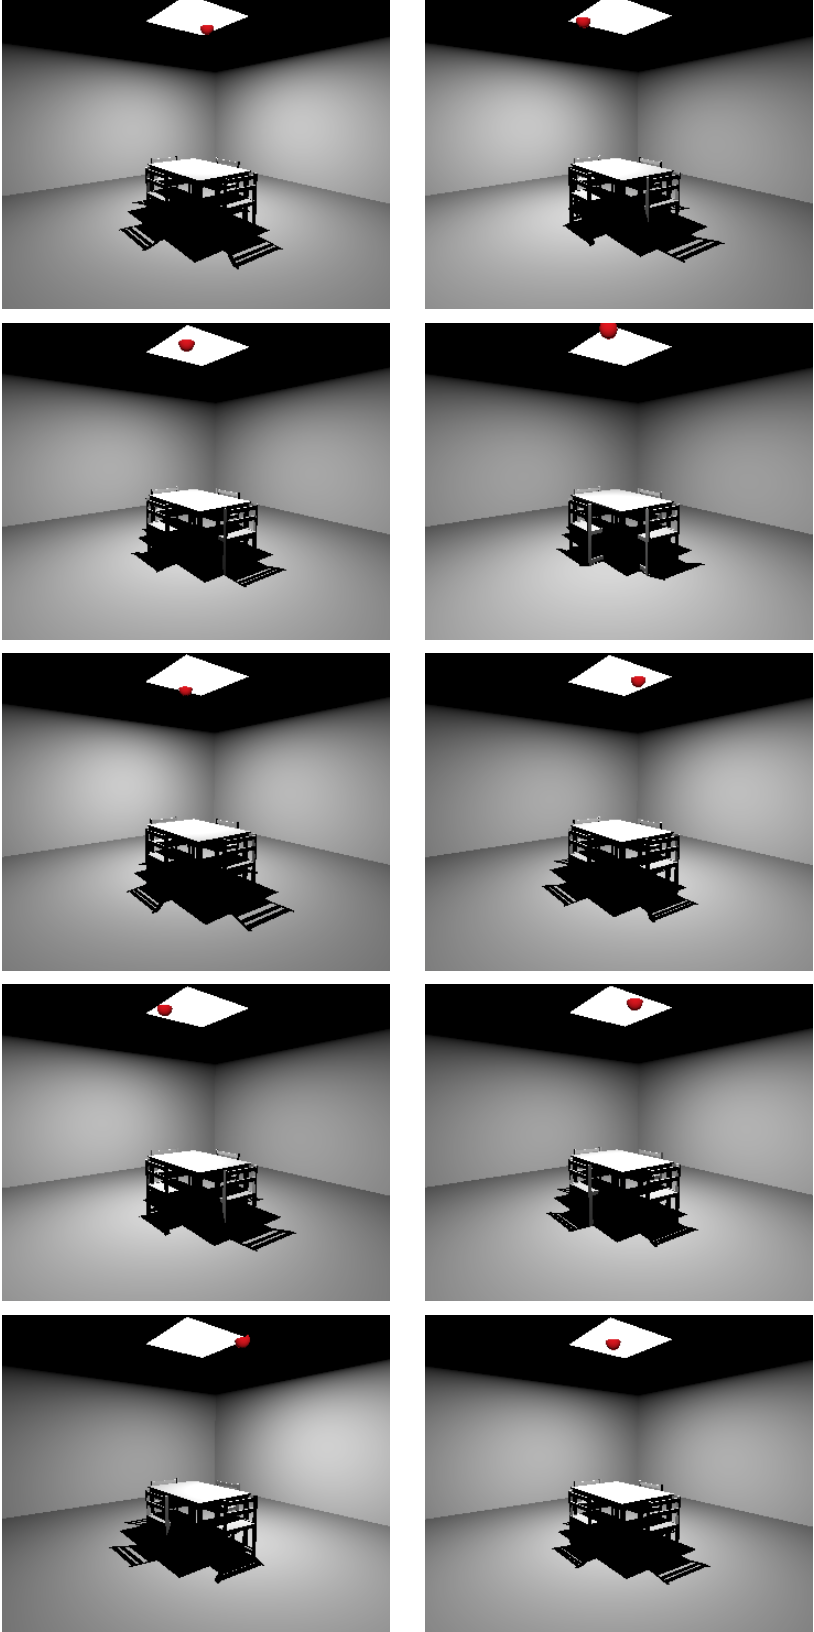
\includegraphics[width=1.0\textwidth]{graphics/ir/ir-1-1}
		\caption{$\langle L_e,\Psi_{mn} \rangle+T_{mn}L_e$}
	\end{subfigure}
	\begin{subfigure}[b]{0.37\textwidth}
		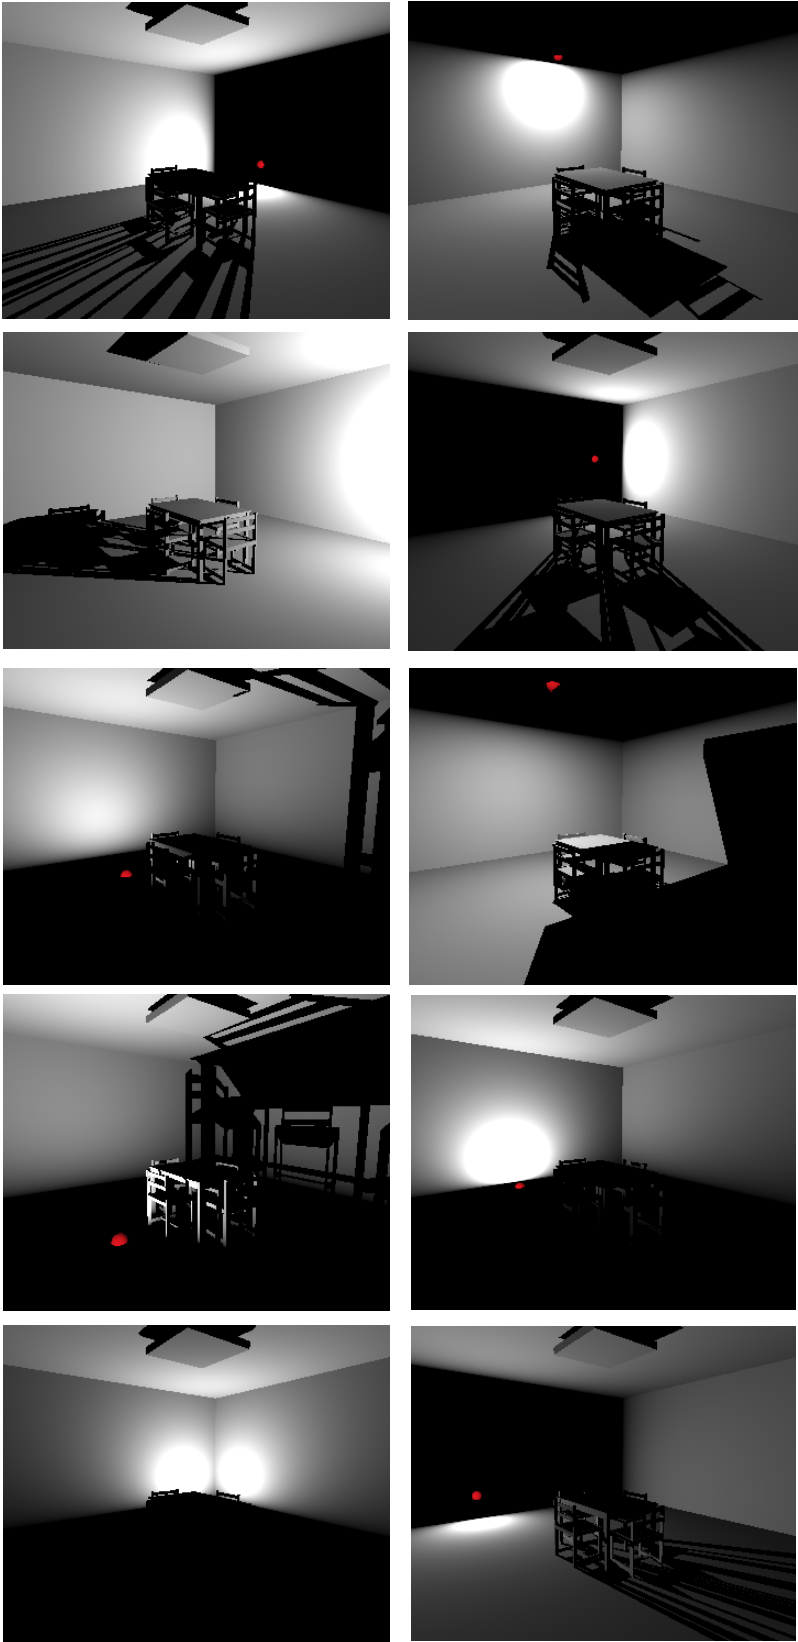
\includegraphics[width=1.0\textwidth]{graphics/ir/ir-1-2}
		\caption{$+T_{mn}T^{n}_{f_d}L$}
	\end{subfigure}
	\begin{subfigure}[b]{0.235\textwidth}
		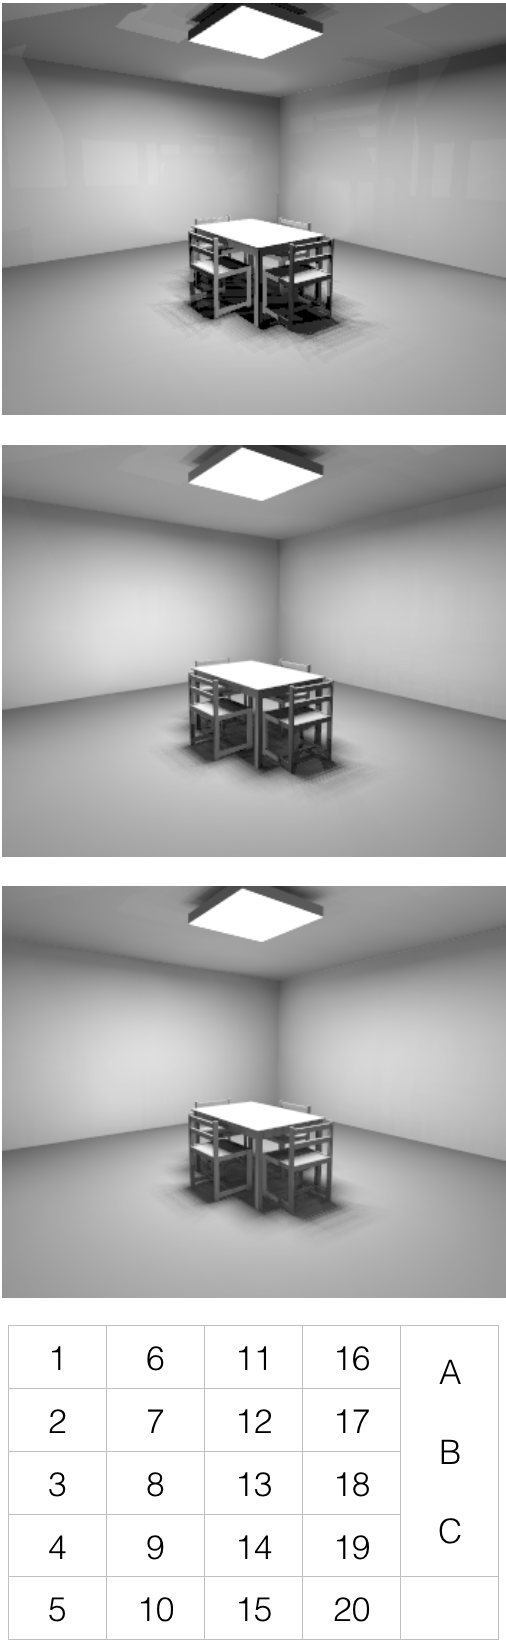
\includegraphics[width=1.0\textwidth]{graphics/ir/ir-1-3}
		\caption{results}
	\end{subfigure}
\end{center}
\caption{Illustration of the quasi-random walk integration scheme showing the intermediate images accumulated for $N=10$ paths with $\overline{\rho}=0.5774$ and the resulting images for $N\in\{ 10,32,64\}$.}
\end{figure*}





\section{Improved Algorithms}
Essentially, instant radiosity is a path tracing technique, more specially a two-pass bidirectional path tracing, which focuses on diffuse lighting and uses quasi-Monte Carlo integration to speedup the computation and convergence of the integration. Because of the low frequency of diffuse lighting, it only needs few sample paths (serval hundreds) to reach a good quality. It is one of the four main techniques of global illumination which can generate high quality images.

Based on instant radiosity or its idea, serval derivations have been introduced. Most of them focus on a rough approximation (such as only one-bounce indirect light) or other more efficient methods to make it can reach interactive even real time performance.  



\subsection{Reflective Shadow Maps}

Temporal Antialiasing in Uncharted 4 pdf
The last of US 那个探照灯





In the origin instant radiosity algorithm, in the light path, every sample particle is emitted like a ray in path tracing. So it needs intersection computation with the scene which is costly. On the other hand, it has been observed that for many purpose, global illumination solution do not need to be precise, but only plausible. Sometimes a rough approximation for the one-bounce indirect light in a scene is enough. 

Based on the above observation, reflective shadow maps\cite{a:ReflectiveShadowMaps}, which introduced by Carsten Dachsbacher et al. in 2005, uses a "shadow map" to represent the indirect point lights. In the first pass, it renders the scene from the view of the light source. The resulting shadow map (a depth buffer) is extended to additionally store the light reflected off the hit surface, which forms a called \textit{reflective shadow map} (RSM). It interprets each of the pixels as a small area light source, that illuminates the scene. In the second pass, it gathers all these pixel lights as the one-bounce indirect light. 



\subsubsection{Data Generation}
A RSM is generated just like a standard shadow map, but with multiple render target: additional to the depth buffer storing the depth buffer value $d_p$, it generates a normal buffer and a world space position buffer with the $n_p$ and $x_p$, and a flux buffer storing $\Phi_p$. Every pixel is interpreted as a \textit{pixel light} that illuminates the scene indirectly. 

\begin{figure}\label{f:rsm-1}
\begin{center}
	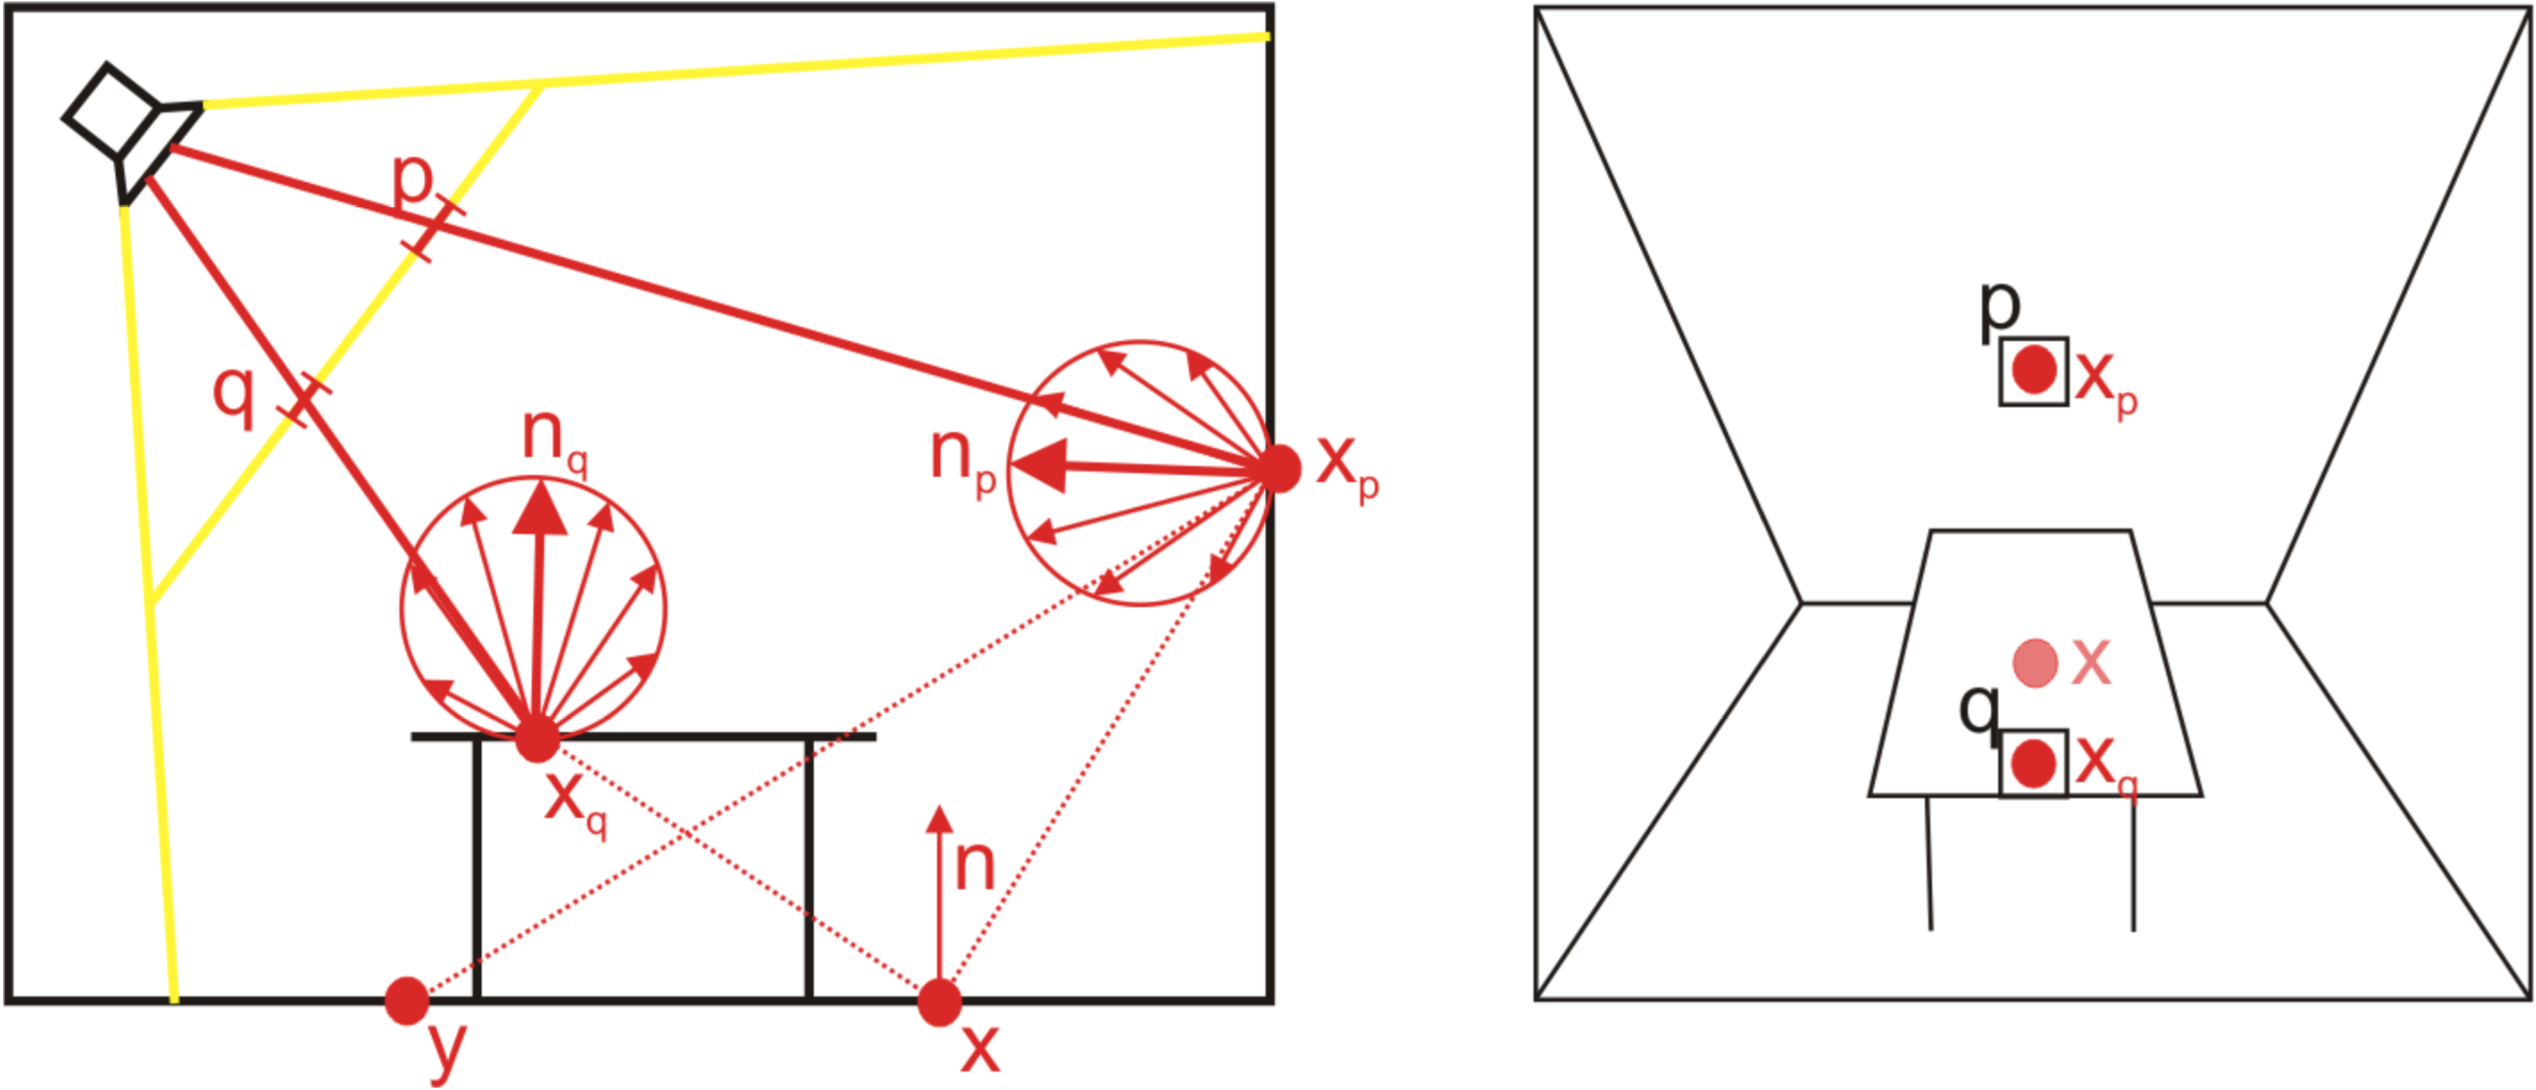
\includegraphics[width=1.0\textwidth]{graphics/ir/ir-2-1}	
\end{center}
	\caption{Two indirect pixel lights $x_p$ and $x_q$ corresponding to two RSM pixels $p$ and $q$.}
\end{figure}

In figure \ref{f:rsm-1}, if we assume that the light source is infinitely small, we can describe the radiant intensity emitted into direction $\omega$ as following by Lambert's cosine law\footnote{\url{https://en.wikipedia.org/wiki/Lambert\%27s_cosine_law}}:

\begin{equation}\label{e:diffuse-radiant-intensity}
	I_p(\omega)=\Phi_p max\{ 0,\langle n_p|\omega \rangle \}
\end{equation}

where $\langle |\rangle$ is the dot product. The irradiance at a surface point $x$ with normal $n$ due to pixel light $p$ is thus:

\begin{equation*}
\begin{aligned}
	E_p(x,n)&=\frac{I_p(\omega)}{r^{r}} \\
			&=\Phi_p\frac{max\{0,\langle n_p|x-x_p \rangle\}max\{0,\langle n|x_p-x \rangle \}}{||x-x_p||^{4}}
\end{aligned}
\end{equation*}

It decided to store radiant flux instead of radiosity or radiance. By this, it doesn't have to care about the representative area of the light, which makes the generation and the evaluation simpler.



\subsubsection{Evaluation}
The indirect irradiance at a surface point $x$ with normal $n$ can be approximated by summing up the illumination due to all pixel lights (Note that it does not consider occlusion for the indirect light sources):

\begin{equation*}
	E(x,n)=\sum_{p}E_p(x,n)
\end{equation*}

Since gathering from all pixels is far too expensive, it has to reduce the sum to a restricted number of light sources. Roughly 300 such samples are necessary to obtain satisfactory results in the examples. They do this using an importance-driven approach, where it tries to concentrate the sampling to the relevant pixel lights.


\begin{figure}\label{f:rsm-2}
\begin{center}
	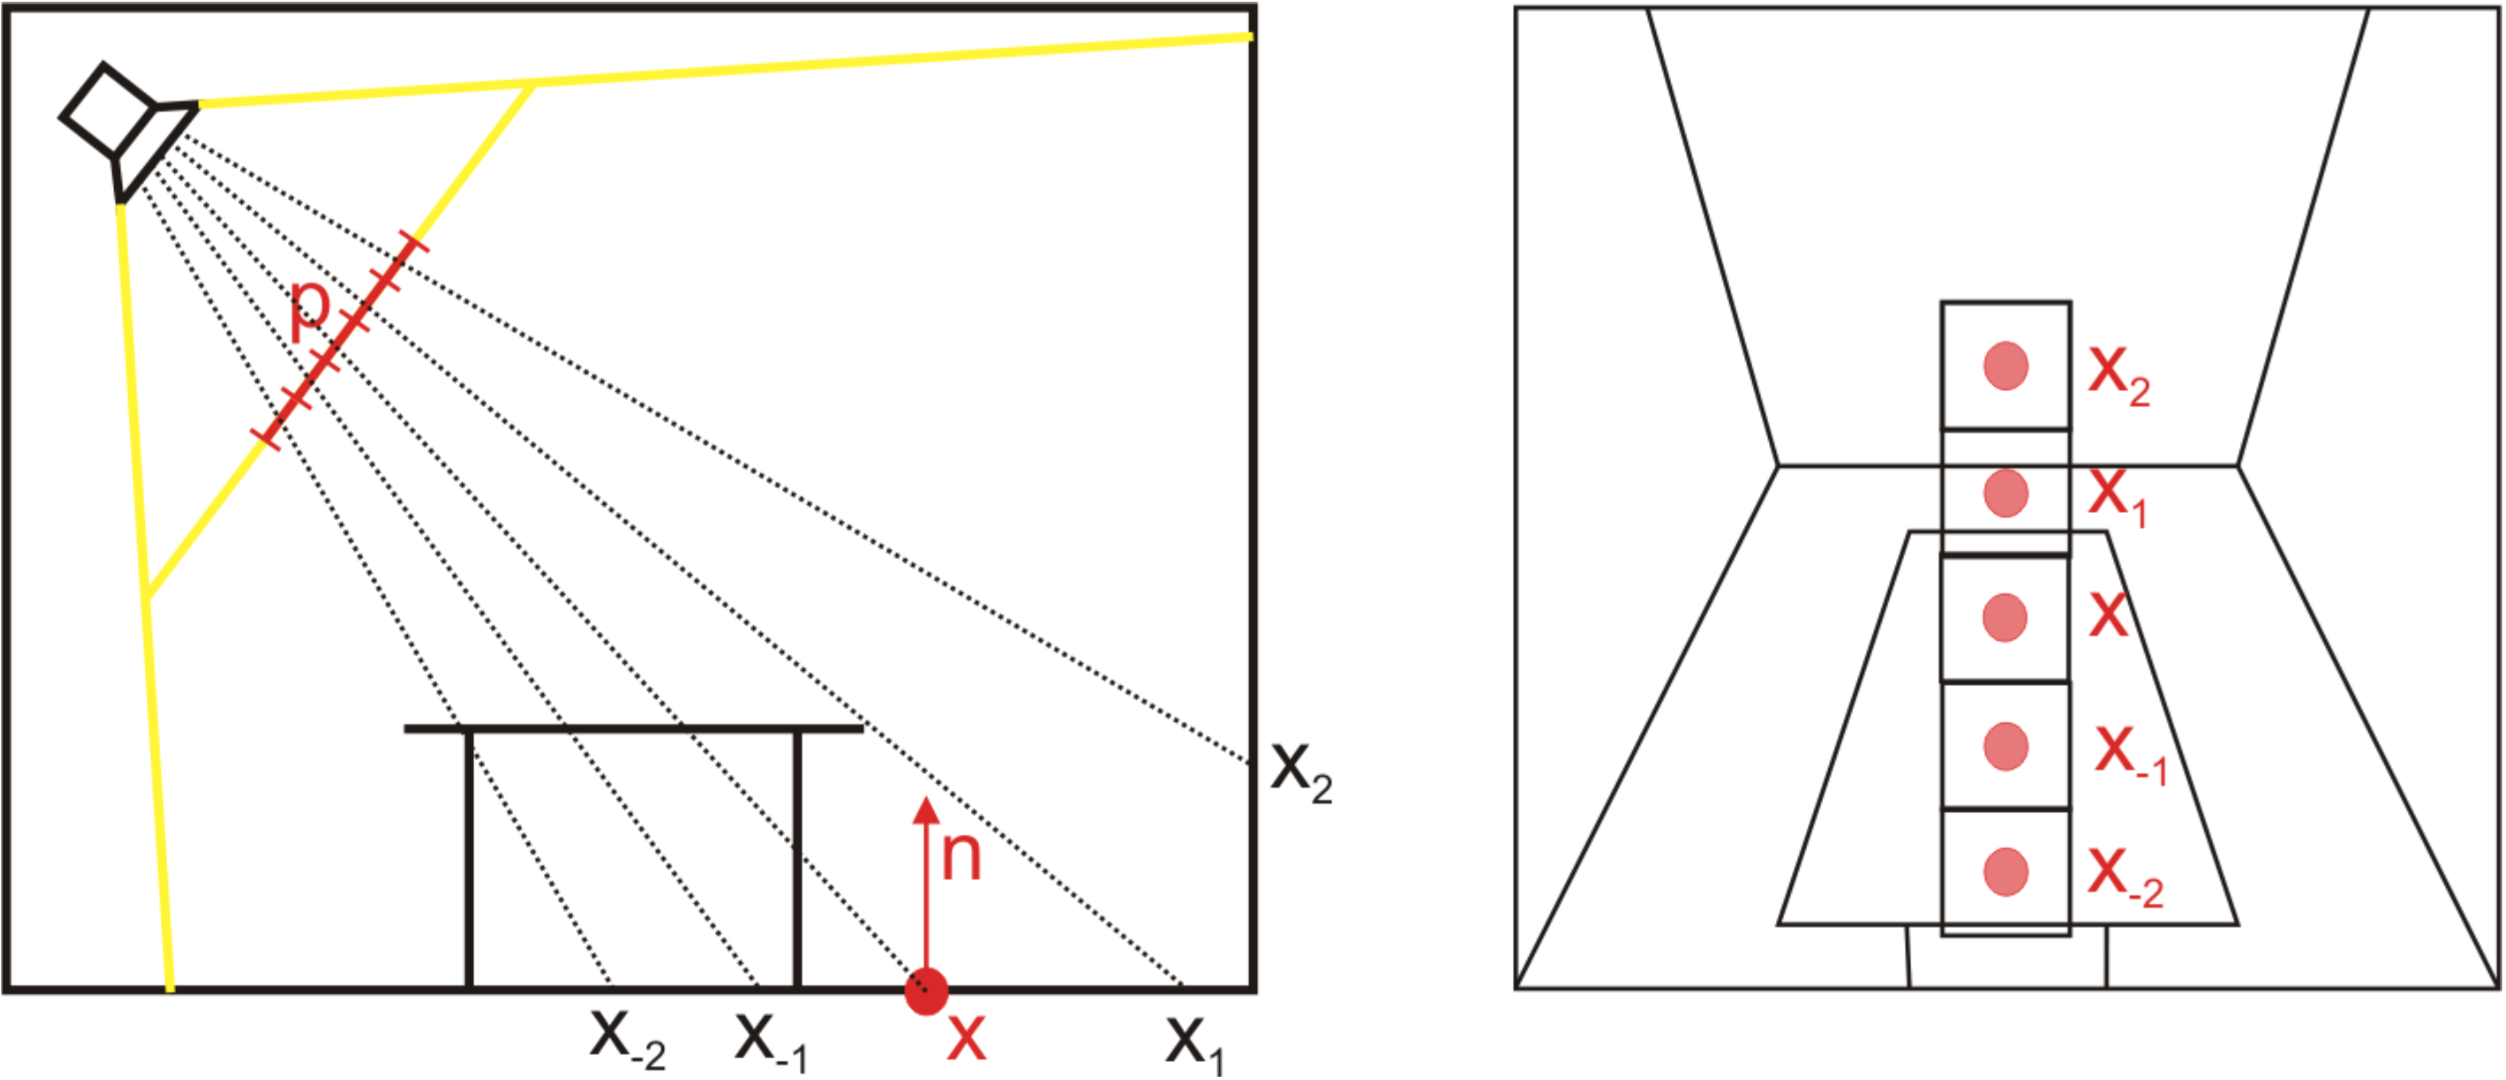
\includegraphics[width=1.0\textwidth]{graphics/ir/ir-2-2}	
\end{center}
	\caption{RSM sampling.}
\end{figure}

The idea can be best described for the example in figure \ref{f:rsm-2}. If we project $x$ into the shadow map, the pixel lights that are closest in world space are also close in the shadow map. The more closer pixel lights has more contribution. Besides, also $x_1$ is very close, but lies on the same plane (floor) as $x$, so it also does not contribute. 

So it decided to obtain the pixel light samples as follows: first, it projects $x$ into the shadow map $(\to (s,t))$. It then selects pixel lights around $(s,t)$, where the sample density decrease with the squared distance to $(s,t)$. This can easily be achieved by selecting the samples in polar coordinates relative to $(s,t)$, i.e. if $\xi_1$ and $\xi_2$ are uniformly distributed random numbers, we select the pixel light at position:

\begin{figure}
\sidecaption
	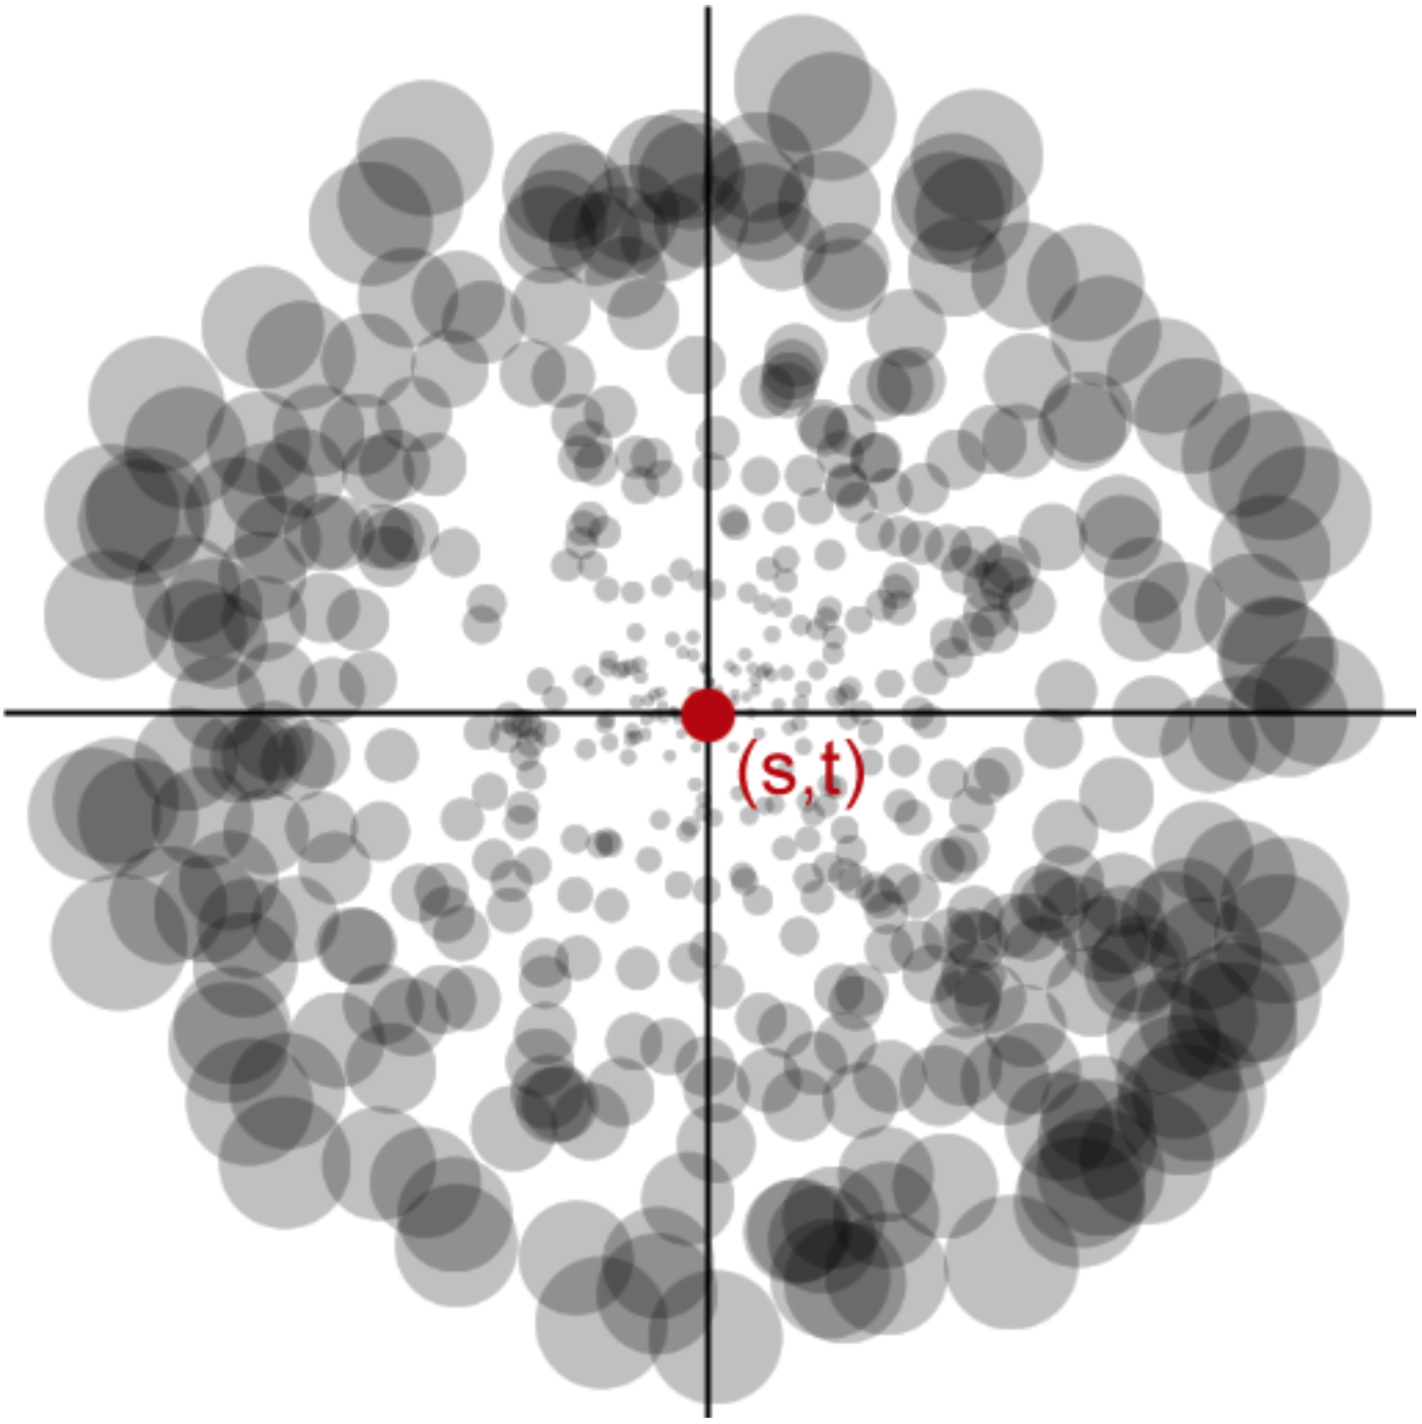
\includegraphics[width=0.65\textwidth]{graphics/ir/ir-2-3}
	\caption{Sampling pattern example. The sample density decreases and the sample weights (visualized by the disk radius) increases with the distance to the center.}
	\label{f:rsm-3}
\end{figure} 


\begin{equation*}
	(s+r_{max}\xi_1 sin(2\pi \xi_2),t+r_{max}\xi_1cos(2\pi\xi_2))
\end{equation*}

It then has to compensate the varying sampling density by weighting the achieved samples with $\xi_1^{2}$ (and a final normalization). An example sampling pattern is shown in figure \ref{f:rsm-3}. In their implementation, they precompute such a sampling pattern and reuse it for all indirect light computations.




\subsubsection{Screen-Space Interpolation}
The indirect lighting computation as described above is still too expensive to be performed for every pixel in an interactive application. So it uses a simple interpolation scheme which can drastically reduce the number of evaluations and use cheap interpolation for the majority of the pixels.

In a first pass, it computes the indirect illumination for a low-resolution image of the camera view. It then renders the full resolution camera view and check for every pixel, whether the indirect light can be interpolated from the four surrounding low-res samples. Such a low-res sample is regarded as suitable for interpolation if the sample's normal is similar to the pixel's normal, and if its world space location is close to the pixel's location. 

\begin{figure}
\sidecaption
	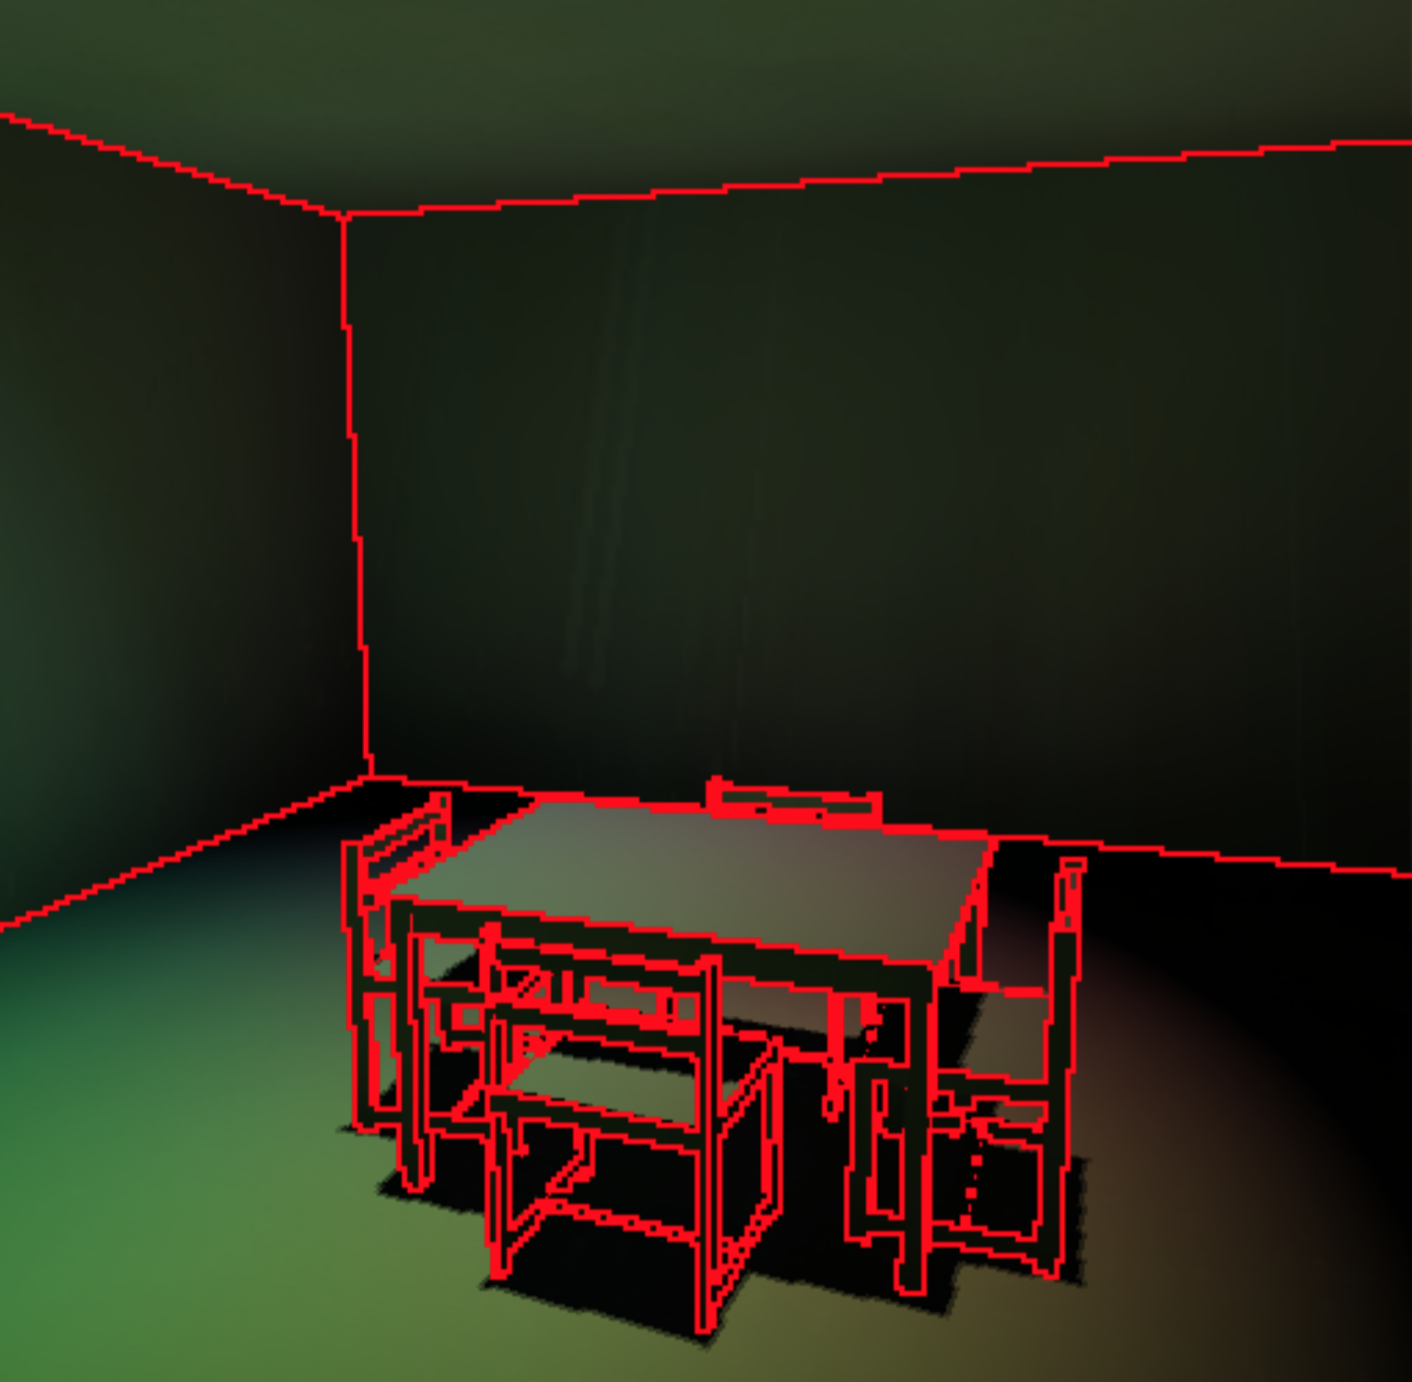
\includegraphics[width=0.65\textwidth]{graphics/ir/ir-2-4}
	\caption{Efficiency of screen space interpolation: only for the red pixels no interpolation was reasonable.}
	\label{f:rsm-4}
\end{figure} 

Each sample's contribution is weighted by the factors used for bi-linear interpolation, including a normalization if not all four samples are used. If three or four samples are considered as suitable, we interpolate the indirect illumination. Otherwise, we discard the pixel in this render pass and rather compute the indirect illumination with the complete gathering step in a final pass.

Figure \ref{f:rsm-4} shows the effectiveness of our solution. Only for the red pixels, interpolation was not sufficient to compute the indirect light. 




\subsection{Splatting Indirect Illumination}
Based on the idea of reflective shadow maps, Carsten Dachsbacher et al. introduced splatting indirect illumination\cite{a:SplattingIndirectIllumination} in 2006. Contrast to RSM, there are three main improvements:

\begin{itemize}
	\item Instead of gathering the indirect light as it is done with RSM, it uses a shooting approach in a deferred shading step. For every indirect light, it splat its contribution into its screen space neighborhood. By this, it can better limit the area of influence of the indirect lights.
	\item An importance sampling strategy, implemented entirely on the GPU, allows efficient selection of secondary light sources.
	\item Furthermore, it can computes indirect lighting from glossy reflectors, which enables us to obtain both indirect diffuse light and caustics in good quality with a unified approach.
\end{itemize}

There are four main steps to do the splatting indirect illumination:

\begin{enumerate}
	\item Create RSM from light position and store the depth value, world position, normal and flux value to texture.
	\item Sample those textures with uniformly distributed sample points.
	\item Render the scene from view position and store world position, normal and surface diffuse color into textures for the later deferred shading.
	\item Each sample point is seen as a virtual point light and do the deferred shading based on these virtual point light.
\end{enumerate} 




\subsubsection{Non-diffuse Surfaces}
To render caustics and indirect illumination from glossy surface, it has to use pixel lights with a non-diffuse emission characteristic. Figure \ref{f:splatting-indirect-illumination-1} compares the emission of the diffuse and glossy pixel lights.

\begin{figure}\label{f:splatting-indirect-illumination-1}
	\begin{center}
		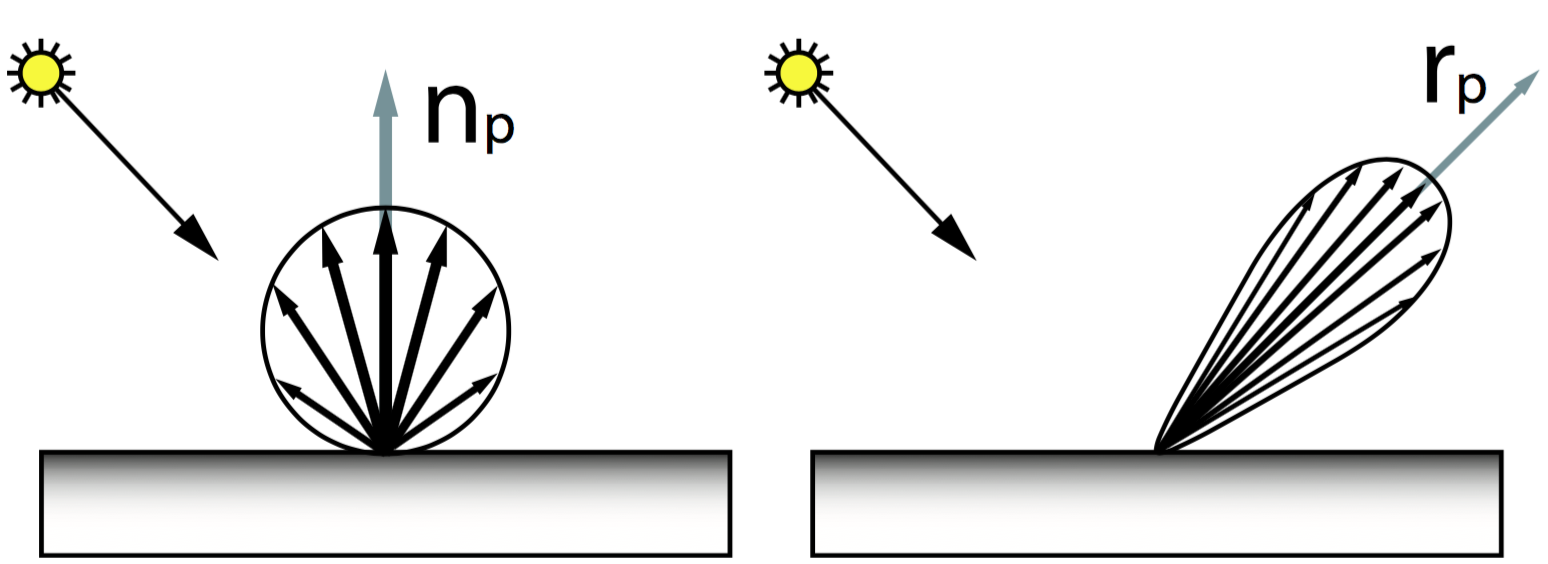
\includegraphics[width=0.7\textwidth]{graphics/ir/ir-3-2}
	\end{center}
	\caption{Emission of diffuse and glossy pixel lights (left and right, respectively).}
\end{figure}

For Phong-like surfaces, the emission of a glossy pixel light $p$ with Phong exponent $P$ is:

\begin{equation}\label{e:non-diffuse-radiant-intensity}
	I_p(\omega)=\Phi_p max\{ 0,\langle r_p|\omega\rangle \}^{P}
\end{equation}

where $r_p$ is main light direction of $p$, which in turn is the reflection direction of light incident at $p$. $r_p$ can be precomputed per glossy pixel light and is then a parameter of the light source such as $P$.

\begin{figure}\label{f:non-diffuse-surfaces}
\begin{center}
	\begin{subfigure}[b]{.48\textwidth}
		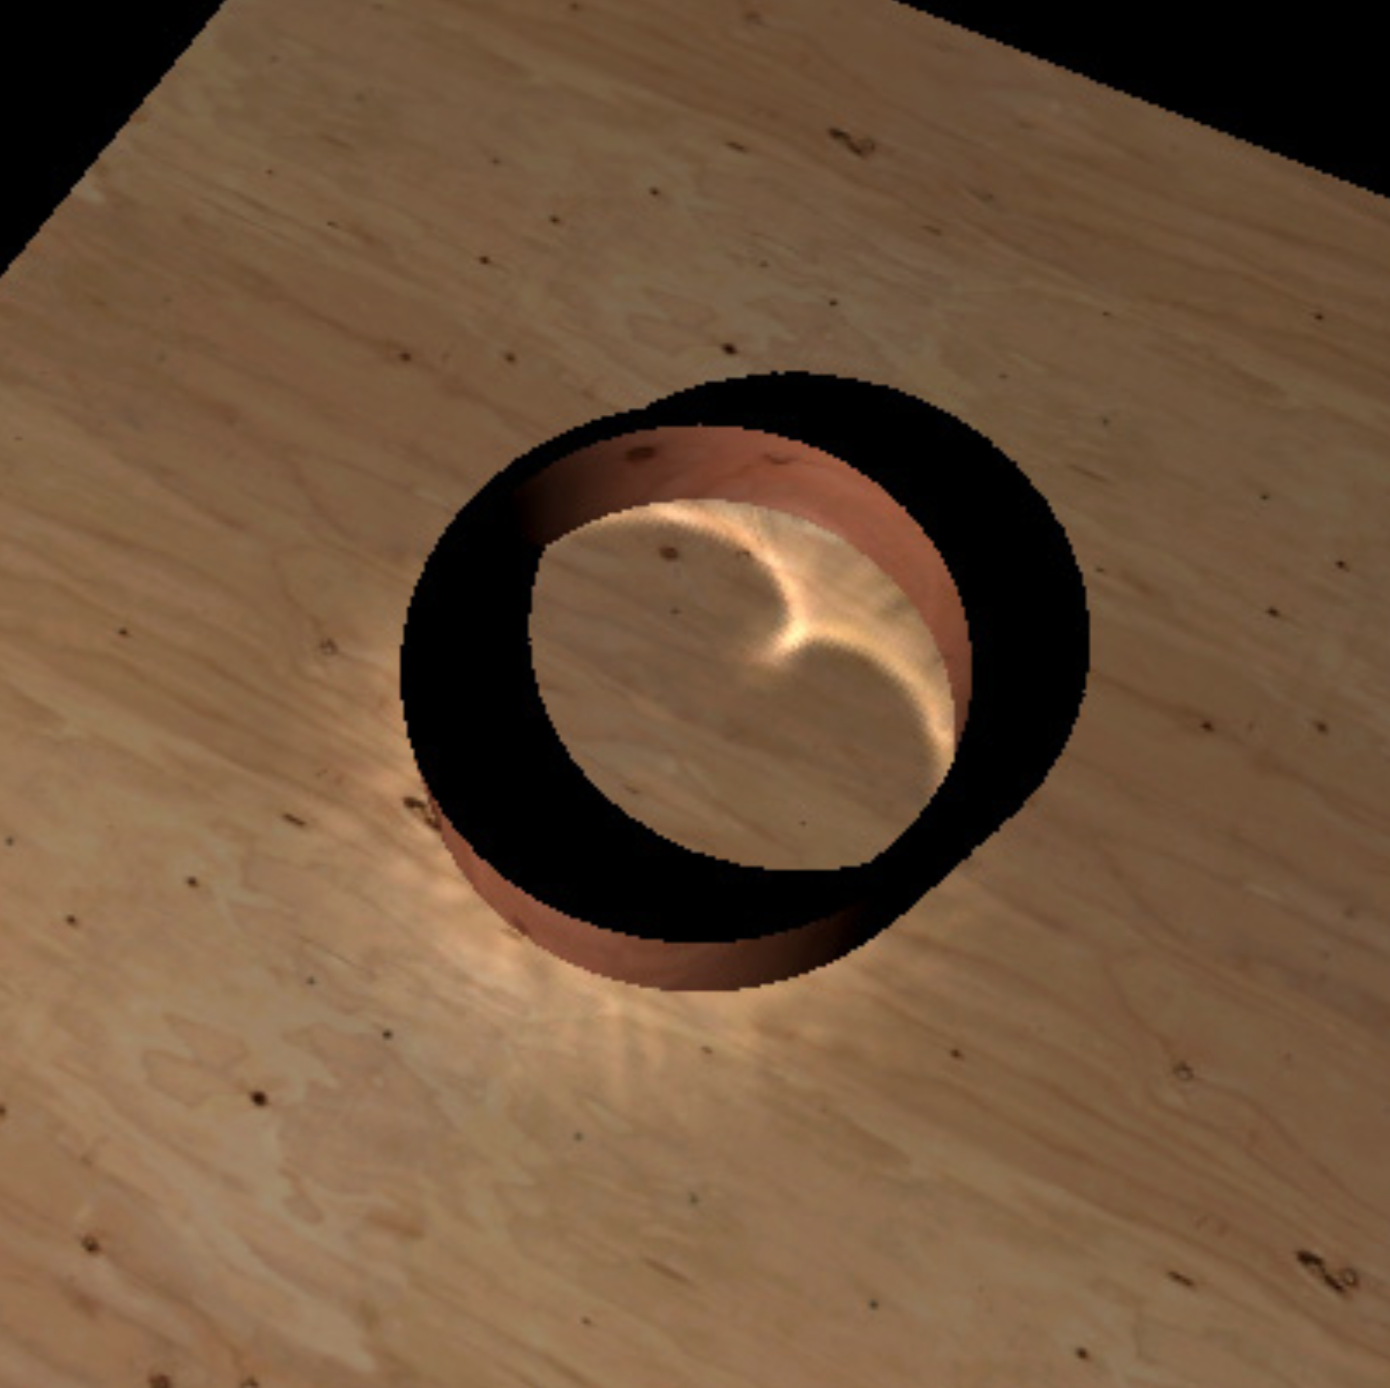
\includegraphics[width=1.\textwidth]{graphics/ir/ir-3-4}
	\end{subfigure}
	\begin{subfigure}[b]{.48\textwidth}
		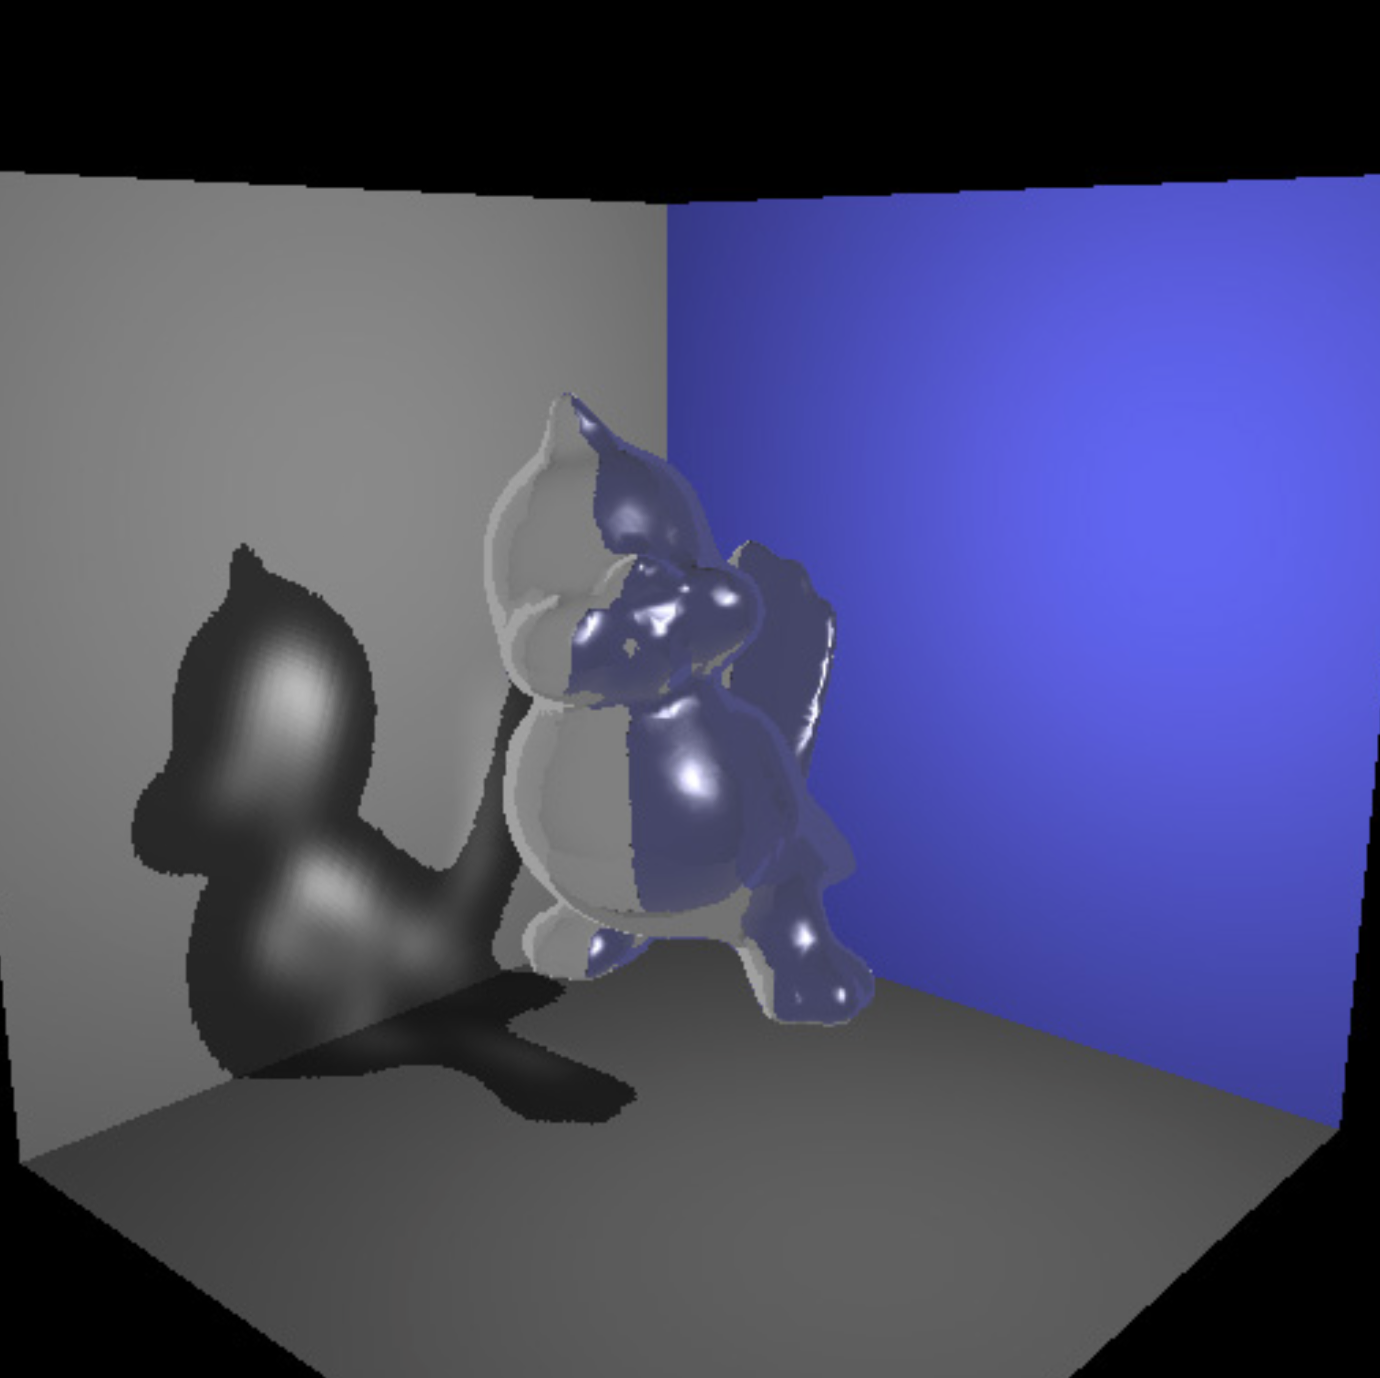
\includegraphics[width=1.\textwidth]{graphics/ir/ir-3-5}
	\end{subfigure}
\end{center}
\caption{A real-time rendering of a metal ring and its caustics on a wood plate at more than 95 frames per second and a refractive glass tweety (only refraction at the back-facing surface) at 150 frames per second.}
\end{figure}

Due to their narrow shape, a screen space quad is a very wasteful approximation for a glossy pixel light. Instead, a tighter bounding geometry is mandatory in this case, as it is described in the next session. With such tight bounds, indirect glossy illumination can be achieved at similar speed as for the diffuse case. Usually, a higher number of glossy pixel lights is necessary, but on the other hand the region of influence is smaller and covers less pixels. Figure \ref{f:non-diffuse-surfaces} shows examples for caustics generated with our approach.




\subsubsection{Importane Sampling}
The importance sampling is particularly important for scenes with non-diffuse surfaces, as these require more samples to approximate their global illumination effects more accurately. They perform an importance sampling as proposed by Clarberg et al\cite{a:WaveletImportanceSampling:EfficientlyEvaluatingProductsofComplexFunctions}. by hierarchical warping. 

As a start, It assumes that the scene consists solely of diffuse surfaces and more samples are to be placed at parts of the scene with higher flux, i.e. as probability distribution it uses the normalized flux.

Each level of the hierarchical warping consists of a vertical and horizontal warping step according to the flux distribution. It begins with a set of uniformly distributed sample points $s_i = (x_i,y_i)^{T},xi , yi \in [0; 1)$ with sample weight $w_i = 1$. Figure \ref{f:splatting-indirect-illumination-2} depicts the warping according to the coarsest level: the initial sample set (Figure \ref{f:splatting-indirect-illumination-2}b) is partitioned into two rows according to the upper and lower average flux ($\Phi_{top}$ and $\Phi_{bottom}$, Figure \ref{f:splatting-indirect-illumination-2}a). The sample points are scaled such that the separation border halves the sample area $[0; 1)^{2}$ (Figure \ref{f:splatting-indirect-illumination-2}c). A new sample point's $y^{'}_i$ is obtained with:

\begin{equation}
	y^{'}_i=\begin{cases}
		y_i/(2\Phi_r) &\text{if }y_i<\Phi_r\\
		(1+y_i-2\Phi_r)/(2(1-\Phi_r)) & \text{otherwise}
	\end{cases}
\end{equation}

where $\Phi_r=\frac{\Phi_{top}}{\Phi_{top}+\Phi_{bottom}}$. To compensate for the varying sampling densities, the sample weights are computed such that the total weight of all samples remains equal:

\begin{equation}
	w^{'}_i=\begin{cases}
		w_i/(2\Phi_r)     & \text{if }y_i<\Phi_r \\
		w_i/(2(1-\Phi_r)) & \text{otherwise}
	\end{cases}
\end{equation}

After the vertical warping, the upper and lower halves are warped analogous to obtain $x^{'}_i$ for each sample (Figure \ref{f:splatting-indirect-illumination-2}d). The warped sampling pattern (Figure \ref{f:splatting-indirect-illumination-2}e) is used to sample the RSM and determine the secondary light sources. The flux taken from the RSM is multiplied with a sample's weight before its contribution to the scene is computed.

\begin{figure*}\label{f:splatting-indirect-illumination-2}
	\begin{center}
		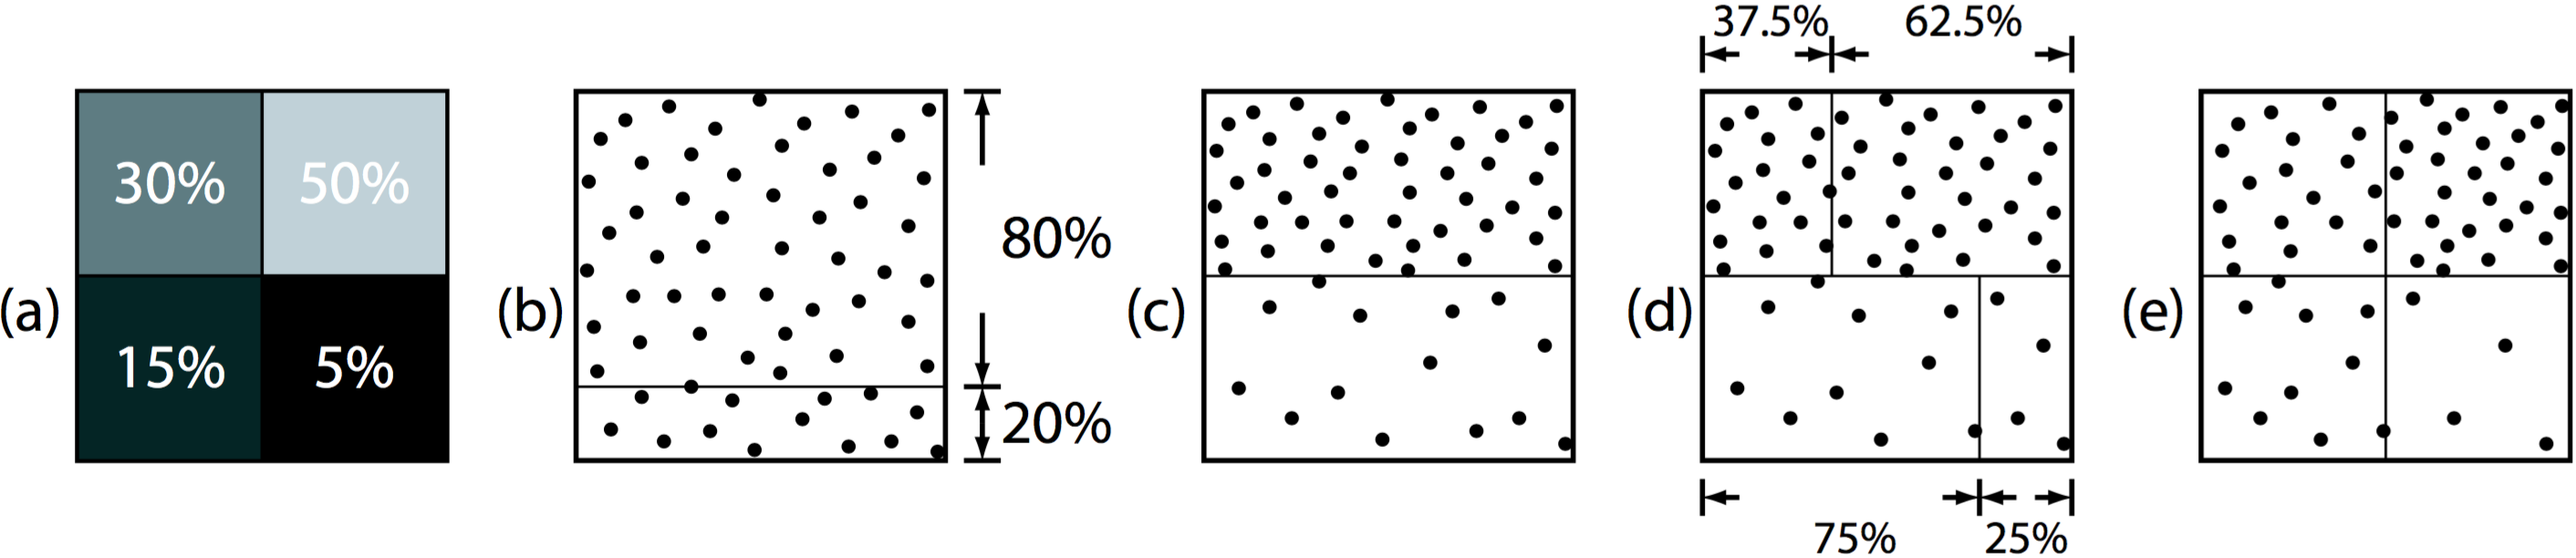
\includegraphics[width=1.0\textwidth]{graphics/ir/ir-3-1}
	\end{center}
	\caption{Importance warping for a single level of the hierarchical importance sampling.}
\end{figure*}

It proposes to perform the importance sampling not just according to the flux, but to a probability distribution obtained from the product of the flux and the maximum value of the BRDF. When using a energy-preserving Phong illumination model, the maximum value of its normalized BRDF is the Phong exponent $P$.

Because the the pixel light doesn't consider occlusion, so an ambient occlusion term $O$ also is considered. To account for the aforementioned heuristics during importance warping, it replaces the flux by the probability: $p_{\Phi} = \Phi\cdot (1 - O) \cdot P$. The corresponding texture storing this term for the light view is called importance sampling buffer and replaces the RSM flux buffer for importance sampling.




\subsubsection{Tighter Bounding Geometry}
In splatting direct illumination, indirect lights only generate significant indirect light in their direct neighborhood. The bounding volume has been carefully designed to tight the sampled point.

The goal is to compute a simple bounded region, outside of which the illumination falls below a threshold $I_{low}$. As one can see in figure \ref{f:splatting-indirect-illumination-3}, for a diffuse pixel light, this region is egg-shaped, and for glossy surfaces the shape is similar to a Phong lobe. Note that these surfaces are iso-surfaces of illumination that include spatial attenuation and are not polar plots of exitant radiance!

For practical reasons, it uses ellipsoids as bounds in both cases. For each pixel light, it has to compute the ellipsoid parameters and it transforms a spherical triangle mesh (with low triangle count) accordingly. 

\begin{figure}\label{f:splatting-indirect-illumination-3}
	\begin{center}
		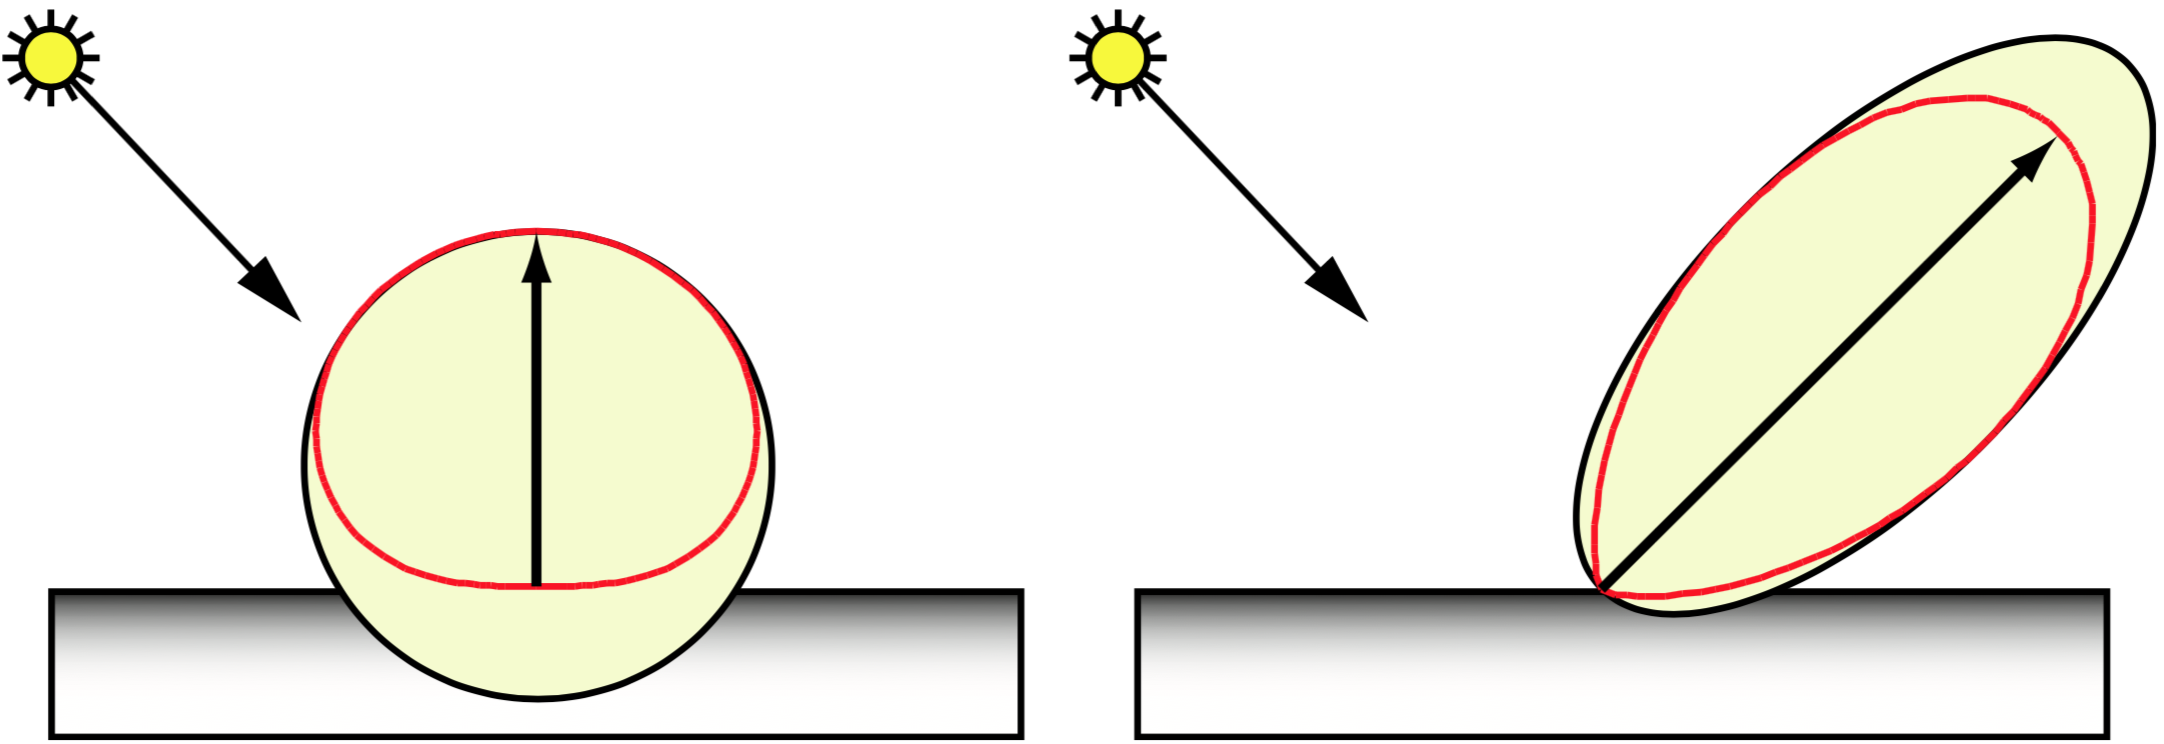
\includegraphics[width=0.7\textwidth]{graphics/ir/ir-3-3}
	\end{center}
	\caption{We adapt the bounding geometry for secondary light sources to reflection properties of the surface. The left image shows a diffuse, the right image a glossy reflection.}
\end{figure}

It is easiest to describe the significant region for a pixel light $p$ in spherical coordinates centered at $p$, i.e. each world-space point is described by a direction $\omega$ and a distance $r$. The irradiance $E$ at a point with polar coordinates $(\omega, r)$ thus depends on: $\omega$, the distance to the light source $r$ and the cosine of the incident angle $\beta$. But since we cannot know $\beta$ in advance, we have to use the bound of one for this term. So we can bound the irradiance at $(\omega,r)$ by $I_p(\omega)/r^{2}$. See figure \ref{f:splatting-indirect-illumination-6}.

\begin{figure}\label{f:splatting-indirect-illumination-6}
	\begin{center}
		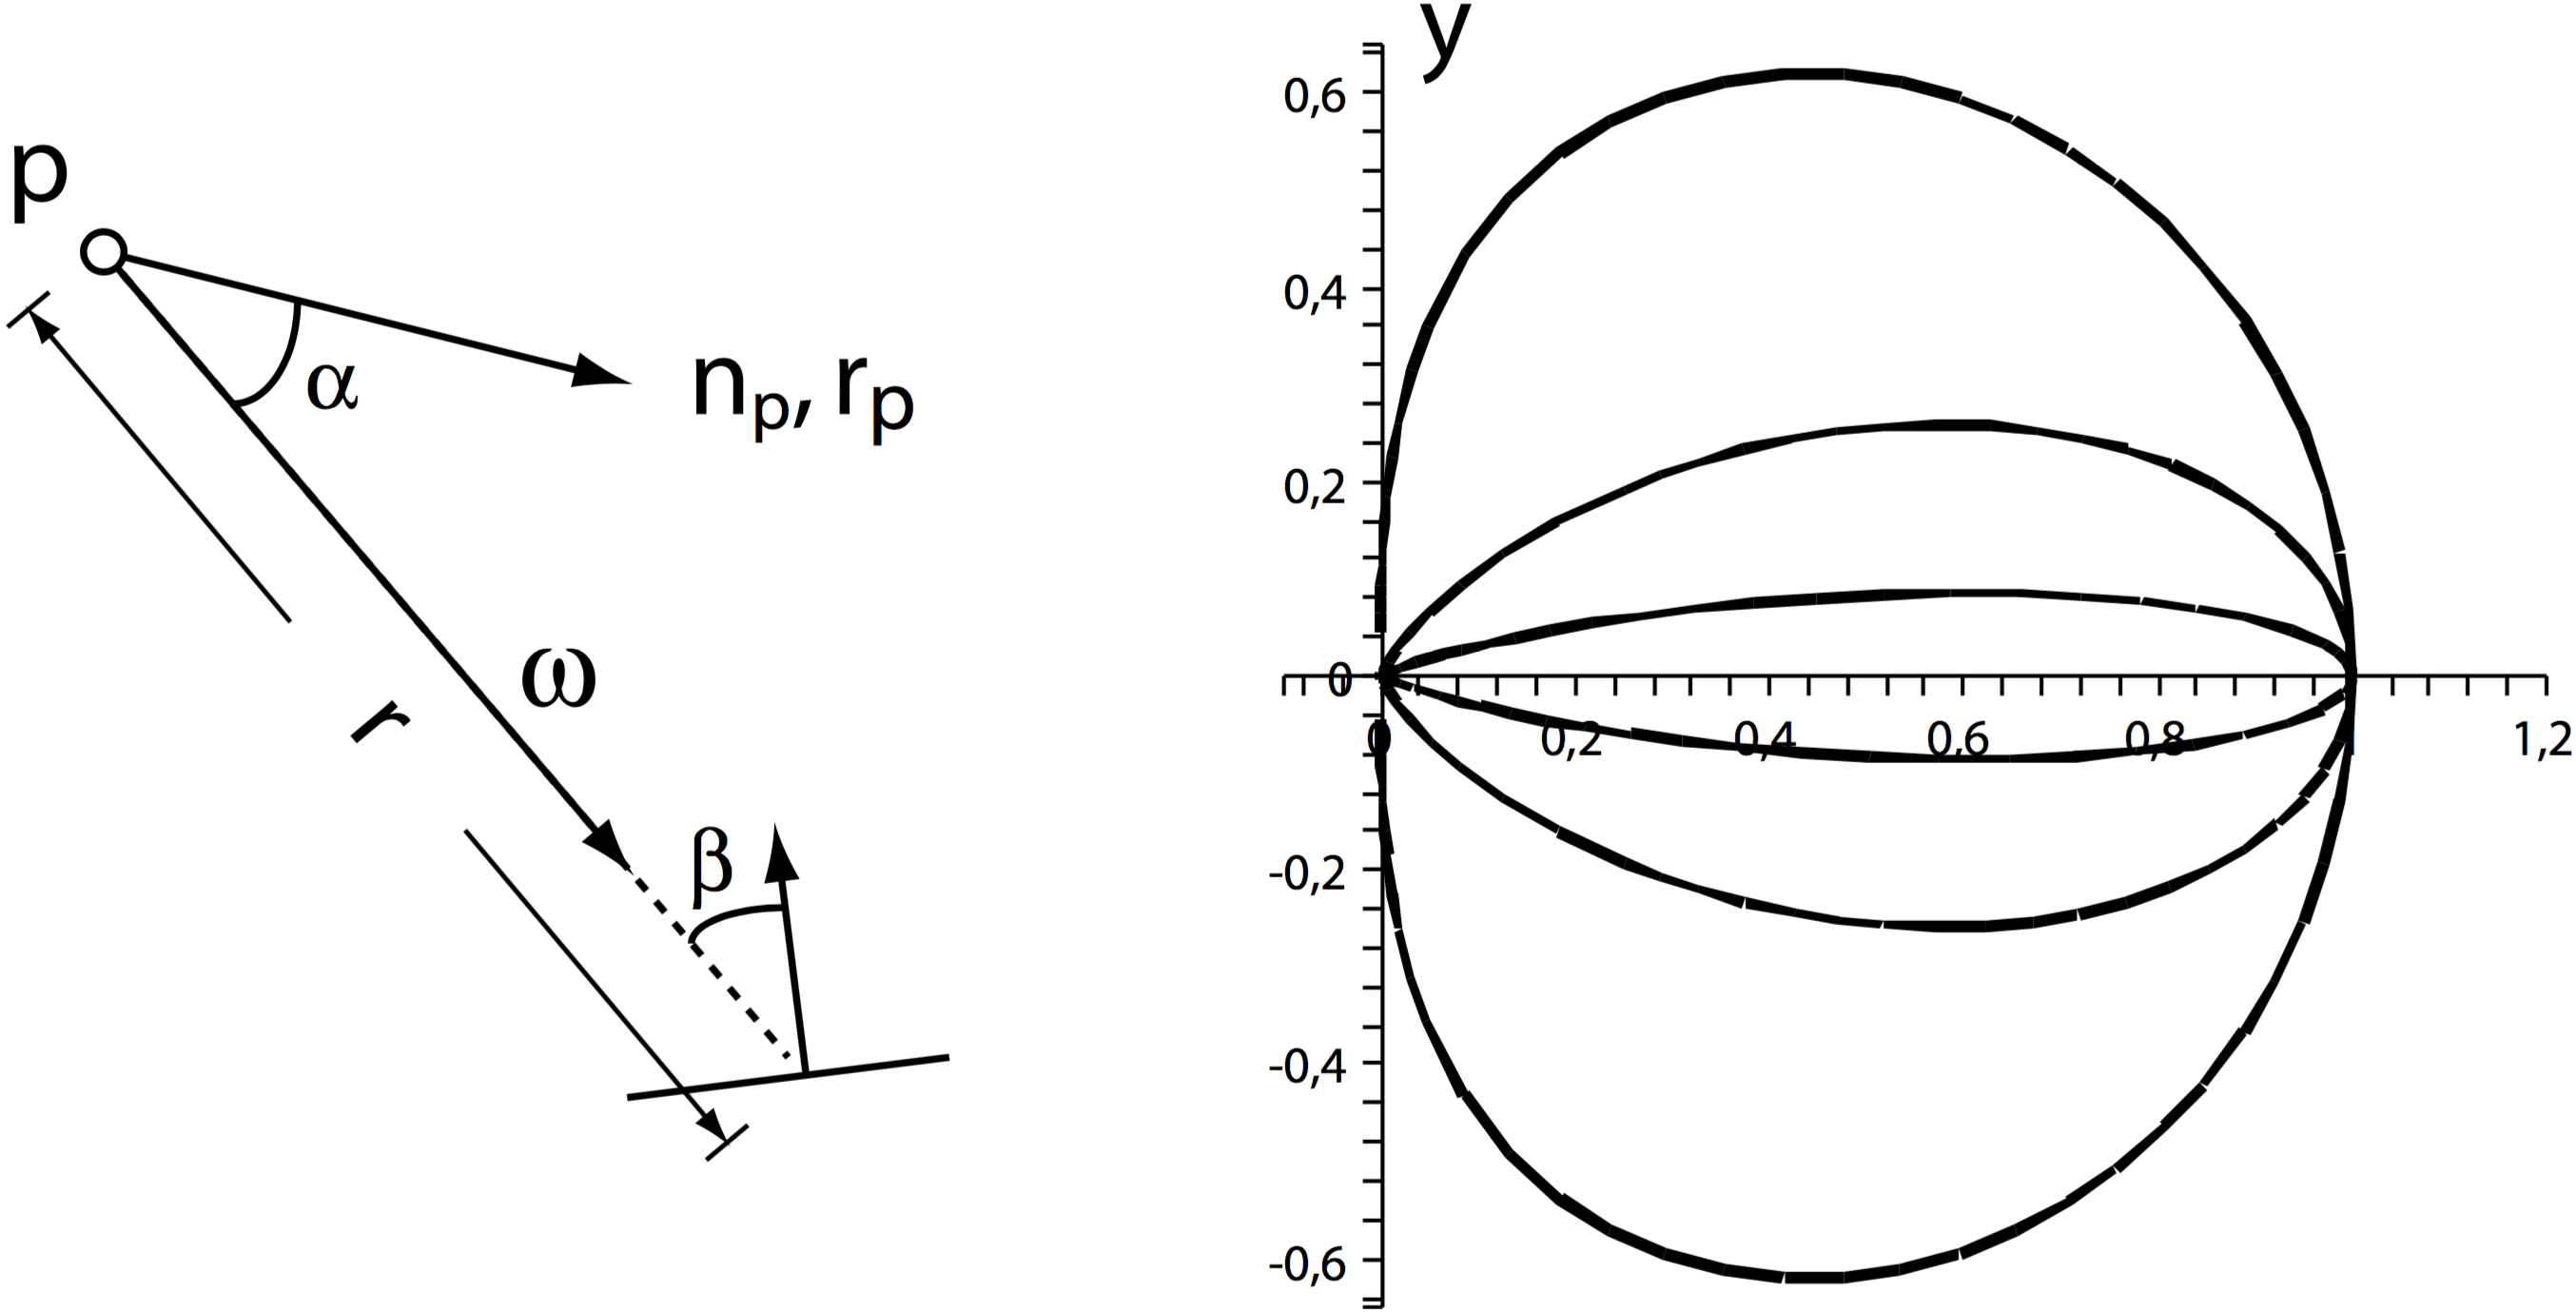
\includegraphics[width=0.8\textwidth]{graphics/ir/ir-3-6}
	\end{center}
	\caption{Left: Illumination computation due to a pixel light. Right: Significant regions for pixel lights with exponents 1, 10, and 100.}
\end{figure}

At this point, it can easily unify diffuse and glossy lights. It denotes as $\alpha$ the angle to the surface normal $n_p$ for diffuse lights (equation \ref{e:diffuse-radiant-intensity}) and the reflection direction $r_p$ for specular lights (equation \ref{e:non-diffuse-radiant-intensity}), see figure \ref{f:splatting-indirect-illumination-1}. If we use an exponent $n = 1$ for diffuse lights, the irradiance can be bound by the 2D polar function $B(\alpha,r) = I_0 cos(\alpha)^{n}/r^{2}$.

The region of influence of $p$ is then bound by the isosurface $B(\alpha,r) = I_{low}$. Figure \ref{f:splatting-indirect-illumination-6} shows the isosurfaces for $I_0 = 1, I_{low} = 1$ and Phong exponents 1, 10, and 100.

Then they fit an ellipse around these shapes with a heuristic which can be seen from the appendix of the original paper. Figure \ref{f:splatting-indirect-illumination-7} shows the isosurfaces in black and the bounding ellipses in gray for $n=1$ and $n=10$.

\begin{figure}\label{f:splatting-indirect-illumination-7}
	\begin{center}
		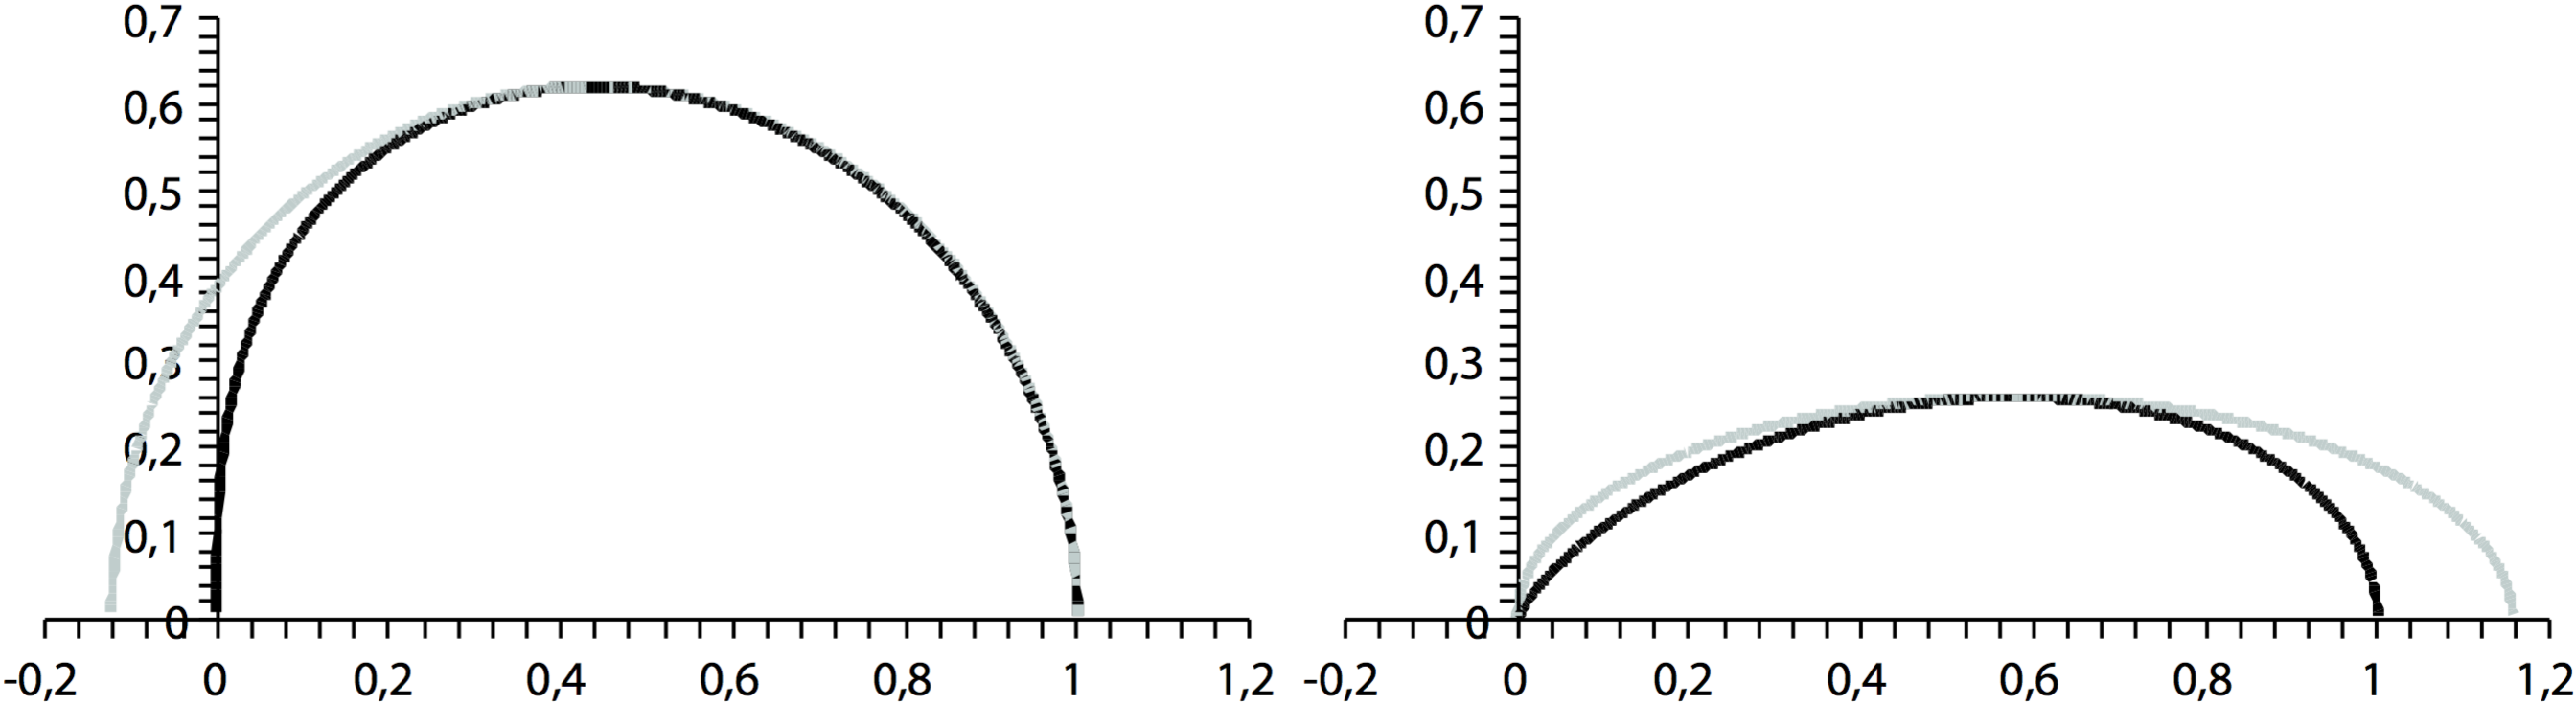
\includegraphics[width=0.9\textwidth]{graphics/ir/ir-3-7}
	\end{center}
	\caption{Isosurfaces and bounds for $n = 1$ and $n = 10$.}
\end{figure}



\subsubsection{Render Final Image}
For the final step, It sees every sampling point as a virtual point light, and send a sphere mesh to the graphics hardware. The fragment shader then computes the contribution for each covered pixel. 





\subsection{Imperfect Shadow Maps}
Shadows of the indirect lights in instant radiosity usually are ignored due to the costly computation. Ambient occlusion (such as \cite{a:DynamicAmbientOcclusionandIndirectLighting}) can be used to account the local visibility. 

T. Ritschel et al. presented a method for interactive computation of indirect illumination in large and fully dynamic scenes based on approximate visibility queries in 2008. They found while the high-frequency nature of direct lighting requires accurate visibility, indirect illumination mostly consists of smooth gradations, which tend to mask errors due to incorrect visibility. They exploit this by approximating visibility for indirect illumination with \textit{imperfect shadow maps} (ISMs)\cite{a:ImperfectShadowMapsforEfficientComputationofIndirectIllumination} --low-resolution shadow maps rendered from a crude point-based representation of the scene.



\subsubsection{Scene Preprocessing}
In a preprocessing step, they approximate the 3D scene by a set of points with roughly uniform density. Each point is created by randomly selecting a triangle with probability proportional to the area of the triangle, and then picking a random location on the triangle. For each point, they also store its barycentric coordinates relative to its triangle as well as the triangle index in order to support dynamic scenes without the need to recompute the point representation. The barycentric coordinates also enable us to retrieve the normal and reflectance for each point, which will be required for secondary indirect light bounces.



\subsubsection{ISM Creation}
A single ISM is created by splatting the point representation into the depth-buffer, where the size of a point splat is based on its squared distance to the corresponding VPL position (assuming each point sample represents the same average area). When an ISM is used for computing indirect illumination, it needs to cover a full hemisphere of depth information (VPLs emit light over a hemisphere) for which it uses parabolic maps.

\begin{figure}\label{f:imperfect-shadow-maps-2}
	\begin{center}
		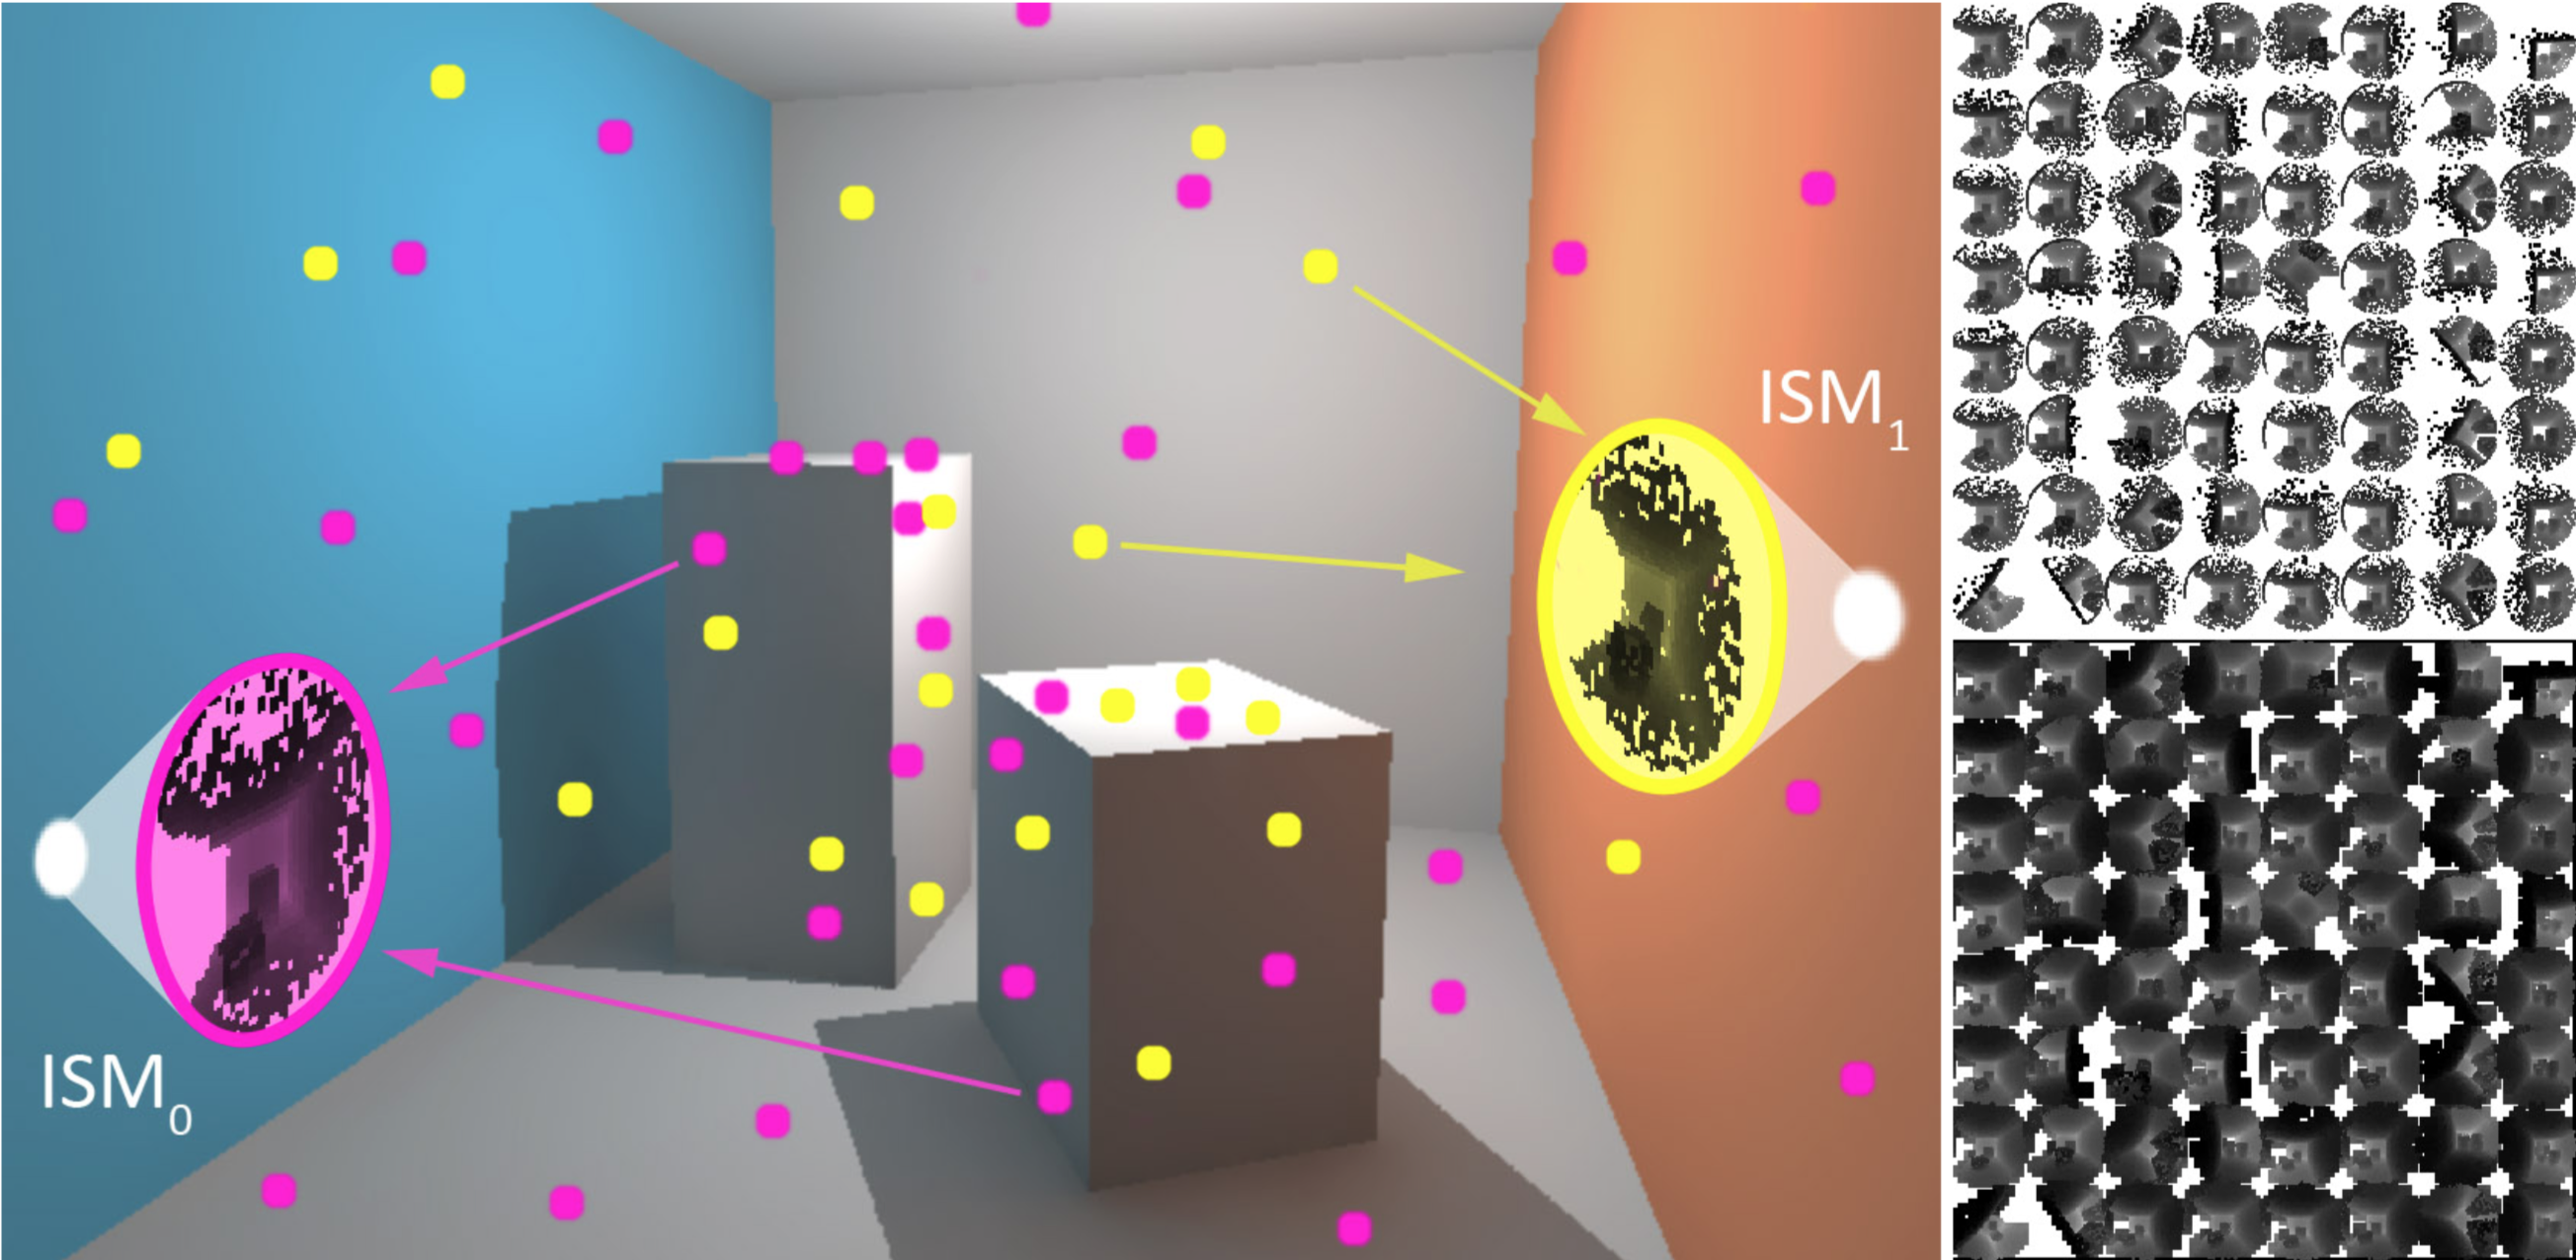
\includegraphics[width=1.\textwidth]{graphics/ir/ir-4-2}
	\end{center}
	\caption{Global Illumination with imperfect shadow maps: The indirect light in this didactic scene is represented by two VPLs. Each VPL generates a shadow map using a point-based representation of the scene. Since coarse visibility information is sufficient, each VPL uses only a sparse subset of the points (encoded as colors) to generate an imperfect shadow map at real-time rates. The contribution of all VPLs is summed up yielding the final indirect illumination. Examples of imperfect shadow maps (bottom with and top without pull-push) are shown on the right; dark value signify small depth values and light values represent large depths.}
\end{figure}

Many low-resolution ISMs are created and rendered in one pass and stored in a single, large texture. To this end, a vertex shader splits up the incoming stream of points representing the scene and distributes an equal amount of points to each ISM within the large texture. Each ISM receives a fixed, random subset of the point set. It typically uses parabolic ISMs with a resolution of $128 \times 128$ pixels, stored in a $4096 \times 4096$ texture. See figure \ref{f:imperfect-shadow-maps-2}.

In order to reduce computation, they only use a sparse set of points, which may leave holes in the depth map. They therefore use a pull-push approach to fill these holes and reconstruct a sensible depth map:

\begin{itemize}
	\item The first step is the creation of an image pyramid in the pull phase where the image is downsampled by a factor of two in each stage. Only valid pixels in the finer level are used for averaging the pixels in the coarser level. 
	\item The second step is the push phase where the holes are filled top-down by interpolating the pixels from the coarser level to approximate the undefined pixels in the finer level. 
\end{itemize}

\begin{figure}\label{f:imperfect-shadow-maps-1}
	\begin{center}
		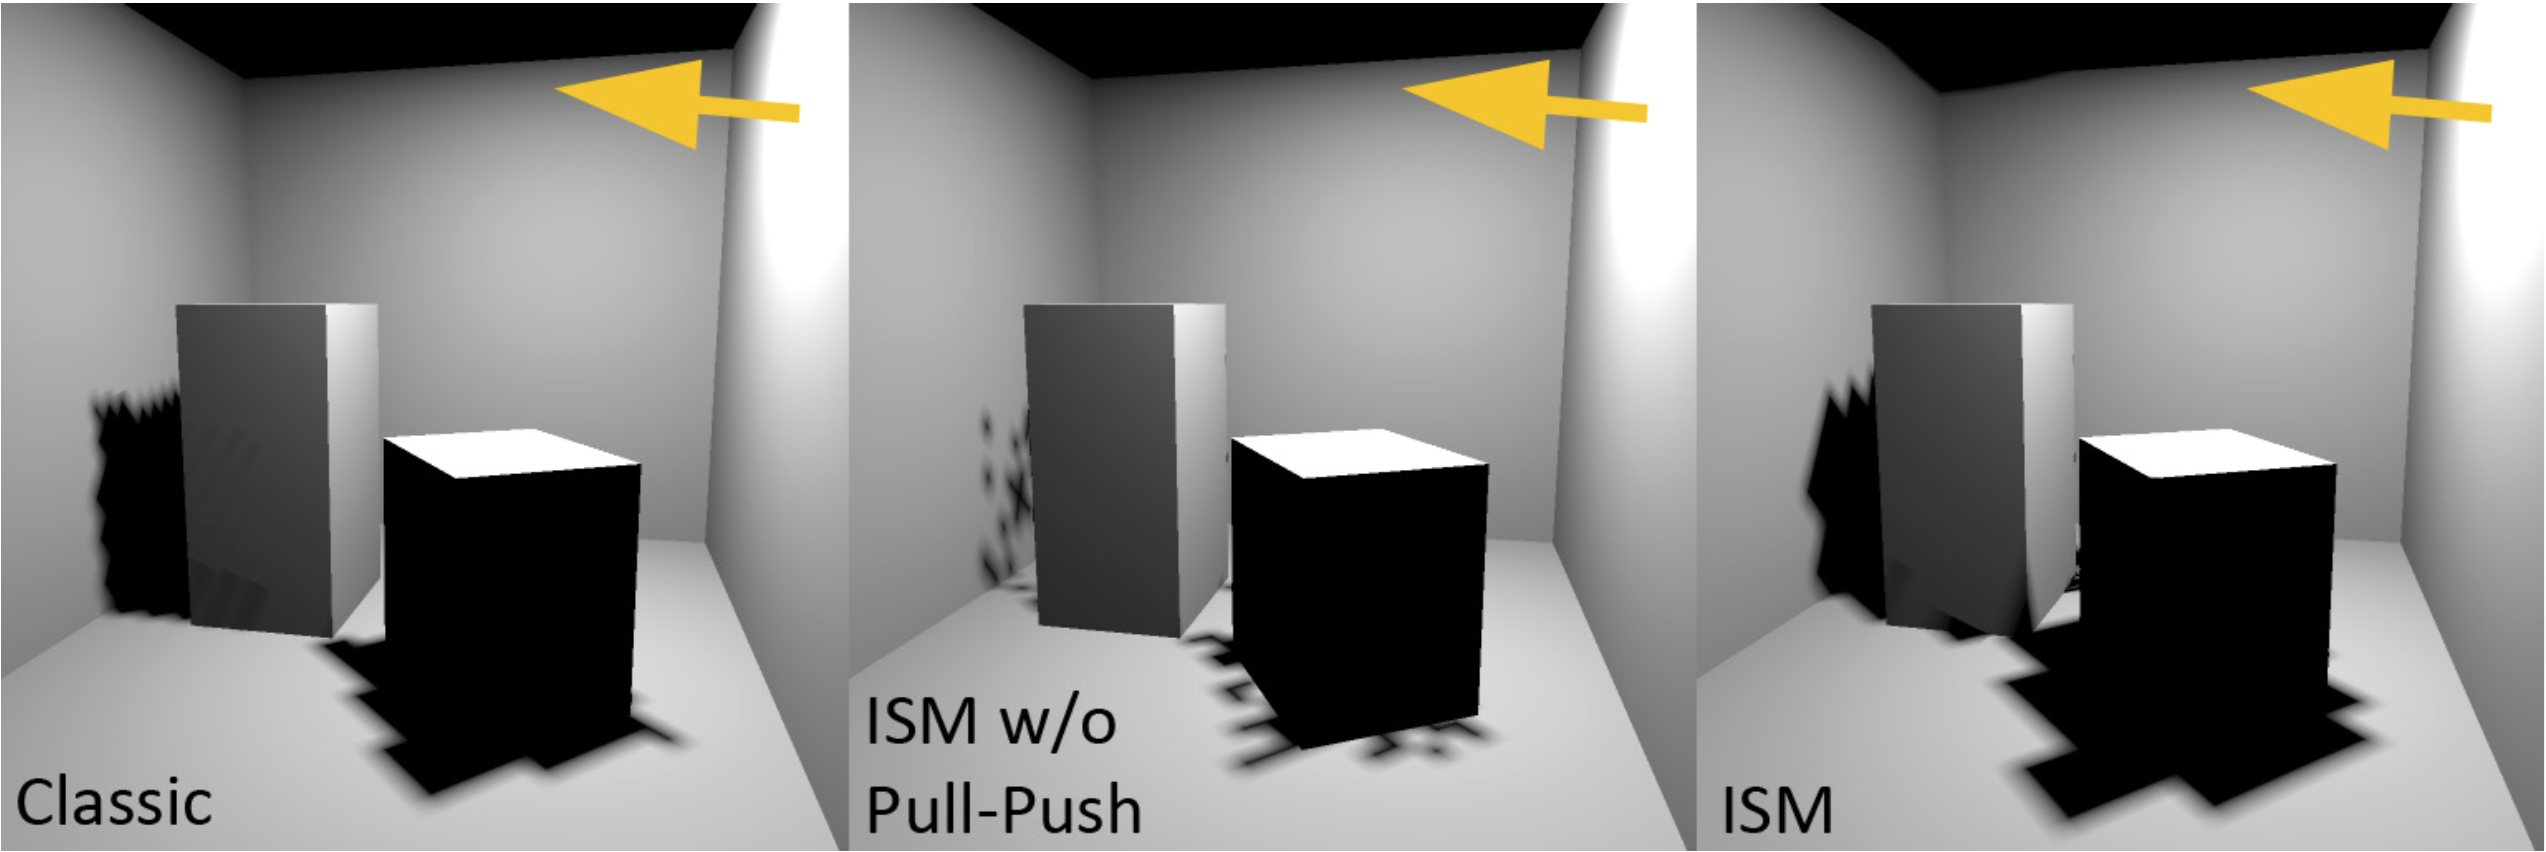
\includegraphics[width=1.\textwidth]{graphics/ir/ir-4-1}
	\end{center}
	\caption{Comparison of a classic shadow map and an imperfect shadow map with and without pull-push. The ISM contains holes and incorrect depth values. Most of these pixels are corrected after the pull-push operation. Note that a single ISM is not expected to produce an accurate shadow. However, shadows from many ISMs average out and artifacts disappear, which is ideal for rendering indirect illumination.}
\end{figure}

They only combine depth values during the pull phase that are close to each other, and they only replace depth values during the push phase that are far from the coarse depth values that are pushed down.


\subsection{Adaptive Imperfect Shadow Maps}
Two main shortcomings exist for ISMs: first, many VPLs are needed, but they are selected without considering the contribution on the final image, leading to the evaluation of many unnecessary candidates. Second, a regular point-based geometry representation can be too coarse to avoid artifacts in large and complex scenes. 

To addresses both issues, Tobias Ritschel et al. introduced view-adaptive imperfect shadow maps\cite{a:MakingImperfectShadowMapsViewAdaptive:HighQualityGlobalIlluminationinLargeDynamicScenes} in 2011. This solution is made view-adaptive by means of two orthogonal improvements: First, the VPL distribution is chosen to provide more detail i. e. more dense VPL sampling, where these contribute most to the current view. Second, the scene representation for indirect visibility is adapted to ensure geometric detail where it affects indirect shadows in the current view.



\subsubsection{Bidirectional RSMs}
To create VPLs, they proposed an approach similar in simplicity and efficiency to RSMs and with the bi-directional ability to focus on relevant VPLs\cite{a:BidirectionalInstantRadiosity}.

First, the scene is rasterized from the current view into a framebuffer ("View" and "Framebuffer" in figure \ref{f:adaptive-ISMs-1}) as well as from the light's point of view into a reflective cube shadow map ("Light" and "RSM" in figure \ref{f:adaptive-ISMs-1}). RSM texels represent \textit{potential} VPLs (pVPL, empty circle in figure \ref{f:adaptive-ISMs-1}). For efficiency, only a subset will be selected as actual VPLs (full yellow circles figure \ref{f:adaptive-ISMs-1}). 

Instead of sampling VPLs based on the outgoing irradiance, they introduced a non-uniform VPL sampling that better estimates the impact on the view samples. To this end, they will not simply use the outgoing radiance, but define a different probability distribution that accounts for the current view ("Bi-dir. imp." in figure \ref{f:adaptive-ISMs-1}).

\begin{figure}\label{f:adaptive-ISMs-1}
	\begin{center}
		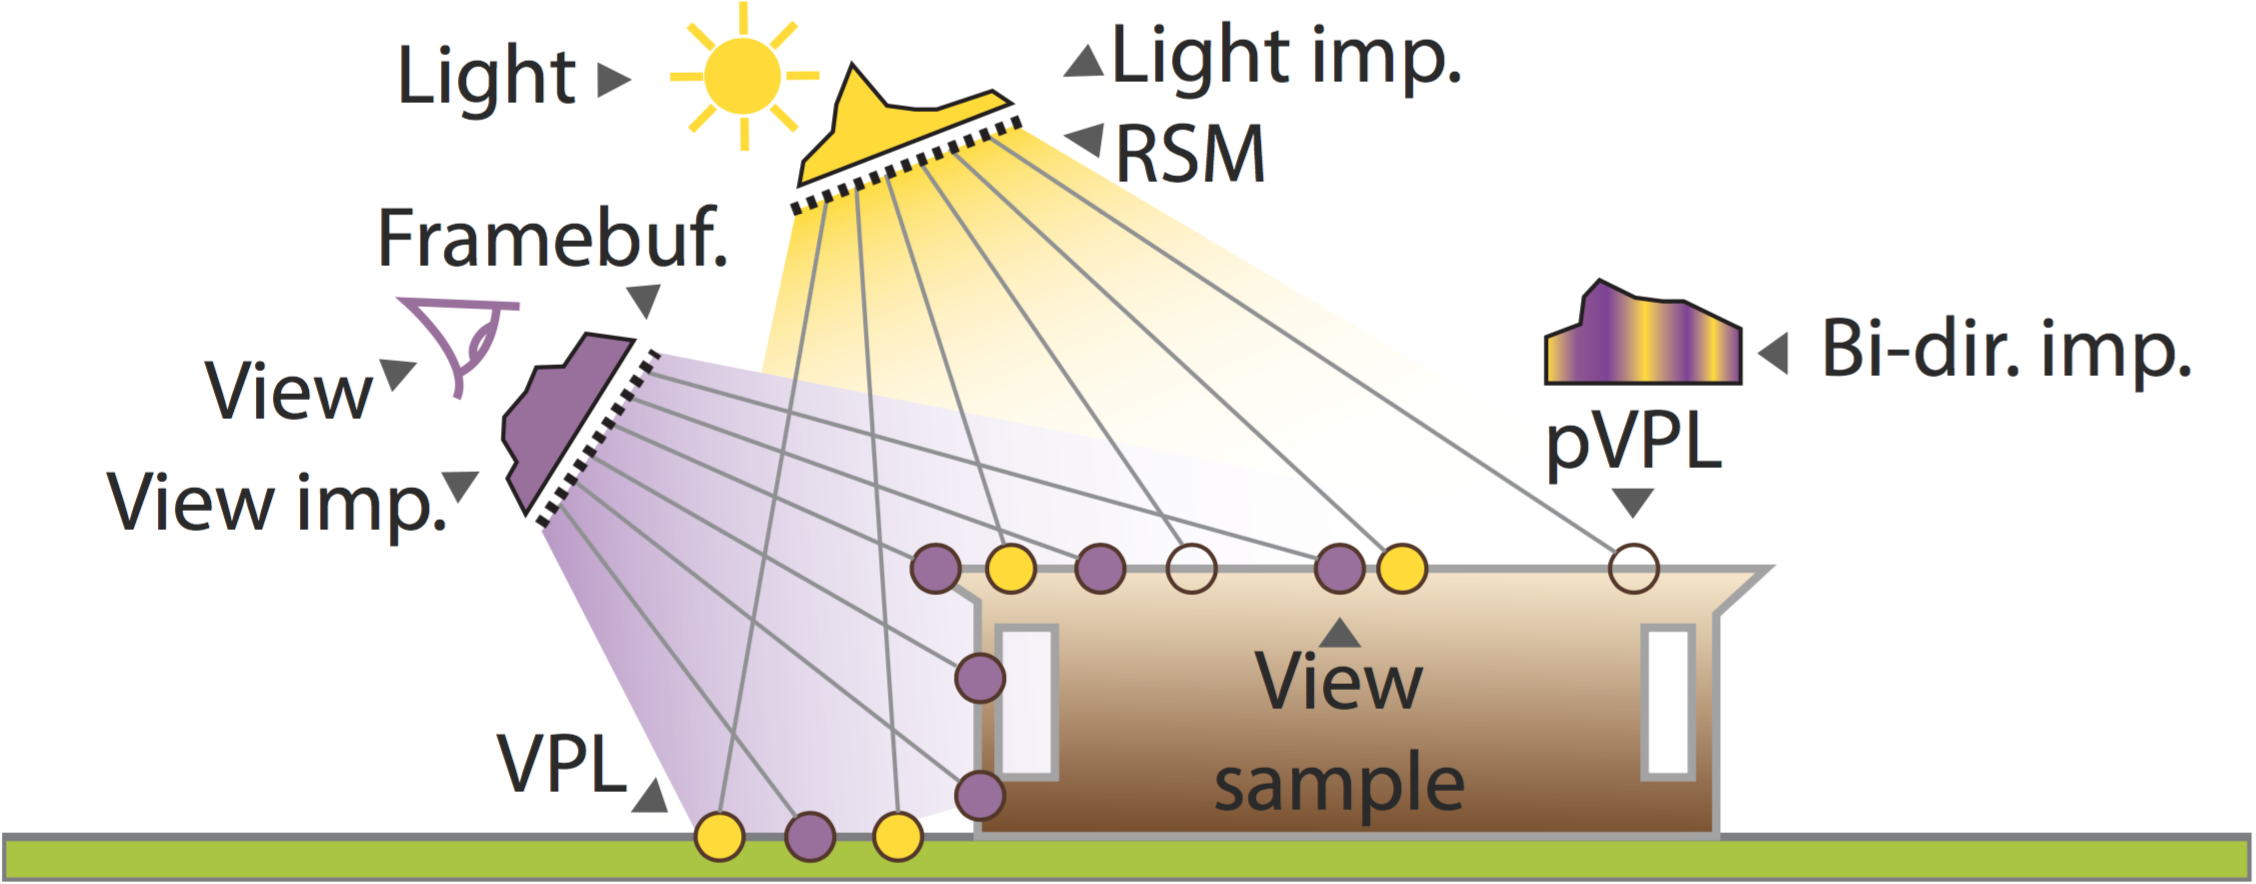
\includegraphics[width=0.7\textwidth]{graphics/ir/ir-5-1}
	\end{center}
	\caption{Bidirectional Reflective Shadow Maps combine importance of direct light and its contribution to the framebuffer.}
\end{figure}

In order to make the approach practical, they introduce two simplifications:

\begin{itemize}
	\item First, they rely on a stochastic solution: each pVPL only evaluates its impact on a few randomly-chosen view samples ($\approx 0.1\%$).
	\item Second, they neglect visibility when evaluating the illumination contribution of each pVPL on the visible scene.
\end{itemize}

Each pVPL's average contribution is then stored in a so-called \textit{Bidirectional Reflective Shadow Map} (BRSM) and VPLs are selected according to this bi-dircetional importance.

To construct the BRSM, each pVPL randomly chooses its view sample set that starts with a regular grid, but jitters the lookup positions which gives good results in practice. 

This paper also introduced a pVPL-dependent importance sampling to guide the view-sample selection to favor those view samples on which the pVPL has the strongest impact. The idea is to exploit the spatial arrangement of the framebuffer. Because view samples correspond to pixels, they are aligned on a grid in image space. Further, two view samples that are close in world space will also be close in the framebuffer. This observation can be used as an estimate. 

Basically, they project the VPL into the current view and then use the screen space distance as an approximation of the world space distance. In other words, a VPL will favor view samples in its vicinity in screen space. They chose a $1/x^{2}$ distance falloff in accordance to the rendering equation. In practice, they clamp the $1/x^{2}$ falloff to $1$ in order to avoid the singularity at $x = 0$.

The efficiency of the solution is illustrated in Figure \ref{f:adaptive-ISMs-3}. Without the guided view-sample selection, most VPLs would choose view samples from the main wall. Hereby increasing the need to perform clamping. Using the guided search, the corner pVPLs on the main wall are likely to find view samples on the side walls. This improves the VPL creation process and the final solution closely resembles the reference rendering while being computationally much cheaper.

\begin{figure}\label{f:adaptive-ISMs-3}
	\begin{center}
		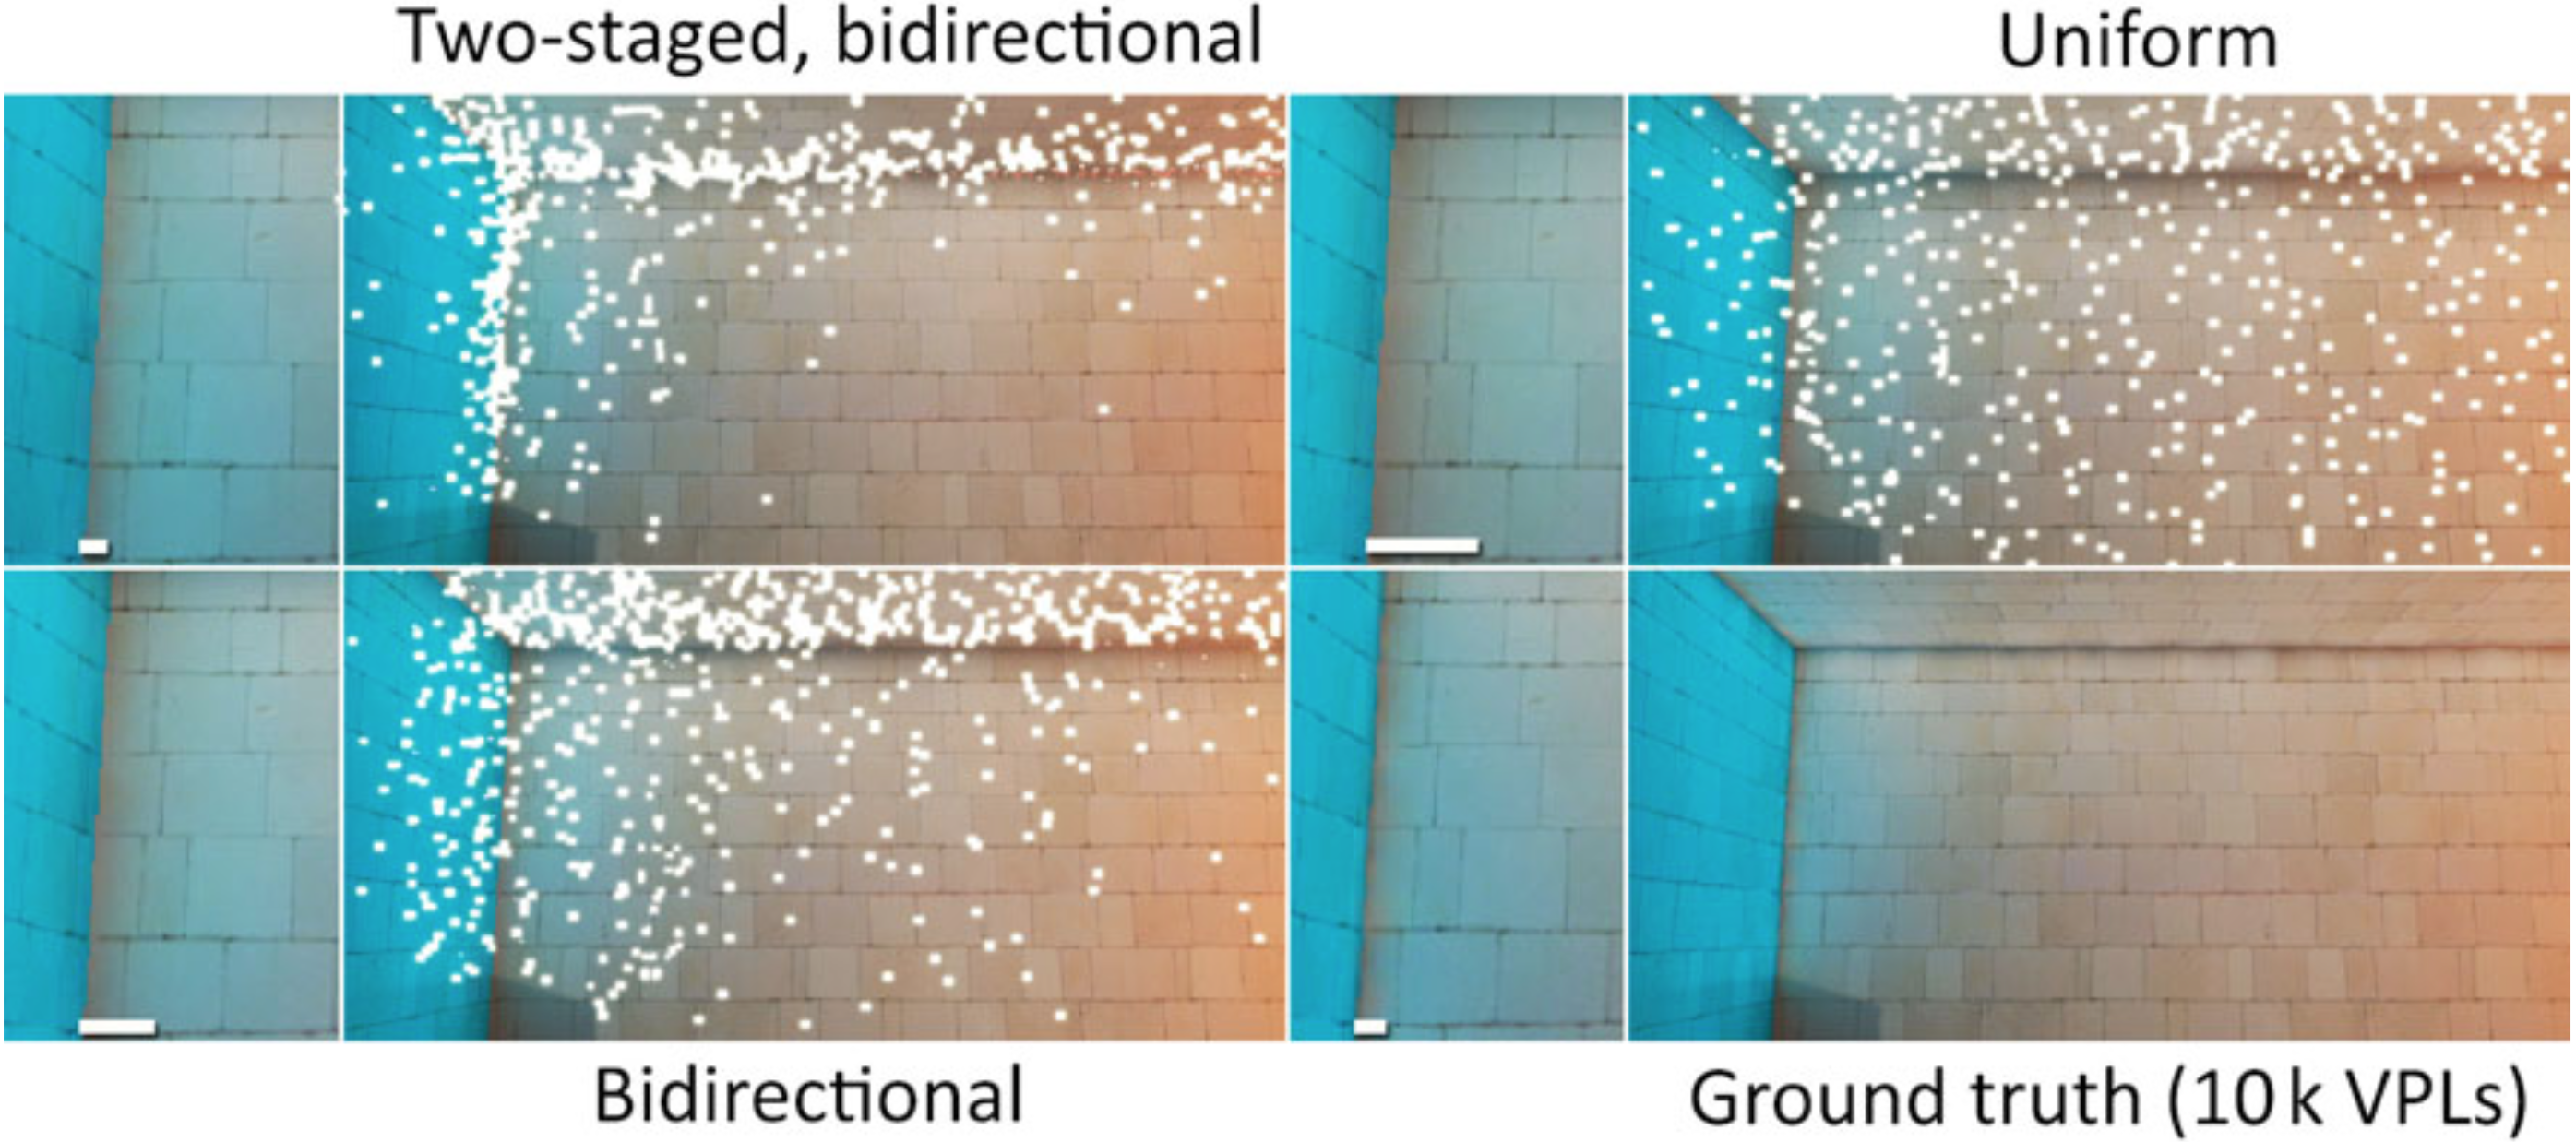
\includegraphics[width=1.\textwidth]{graphics/ir/ir-5-3}
	\end{center}
	\caption{A comparison of various estimation strategies for the VPL sampling. A comparison with a ground truth shows how better sampling strategies deliver more faithful results. The white bar denotes the bias due to clamping in each solution: Smaller is better.}
\end{figure}


In order to choose VPLs according to the distribution density by the BRSM, it will rely on several \textit{cumulative density functions} (CDFs).

\begin{figure}\label{f:adaptive-ISMs-2}
	\begin{center}
		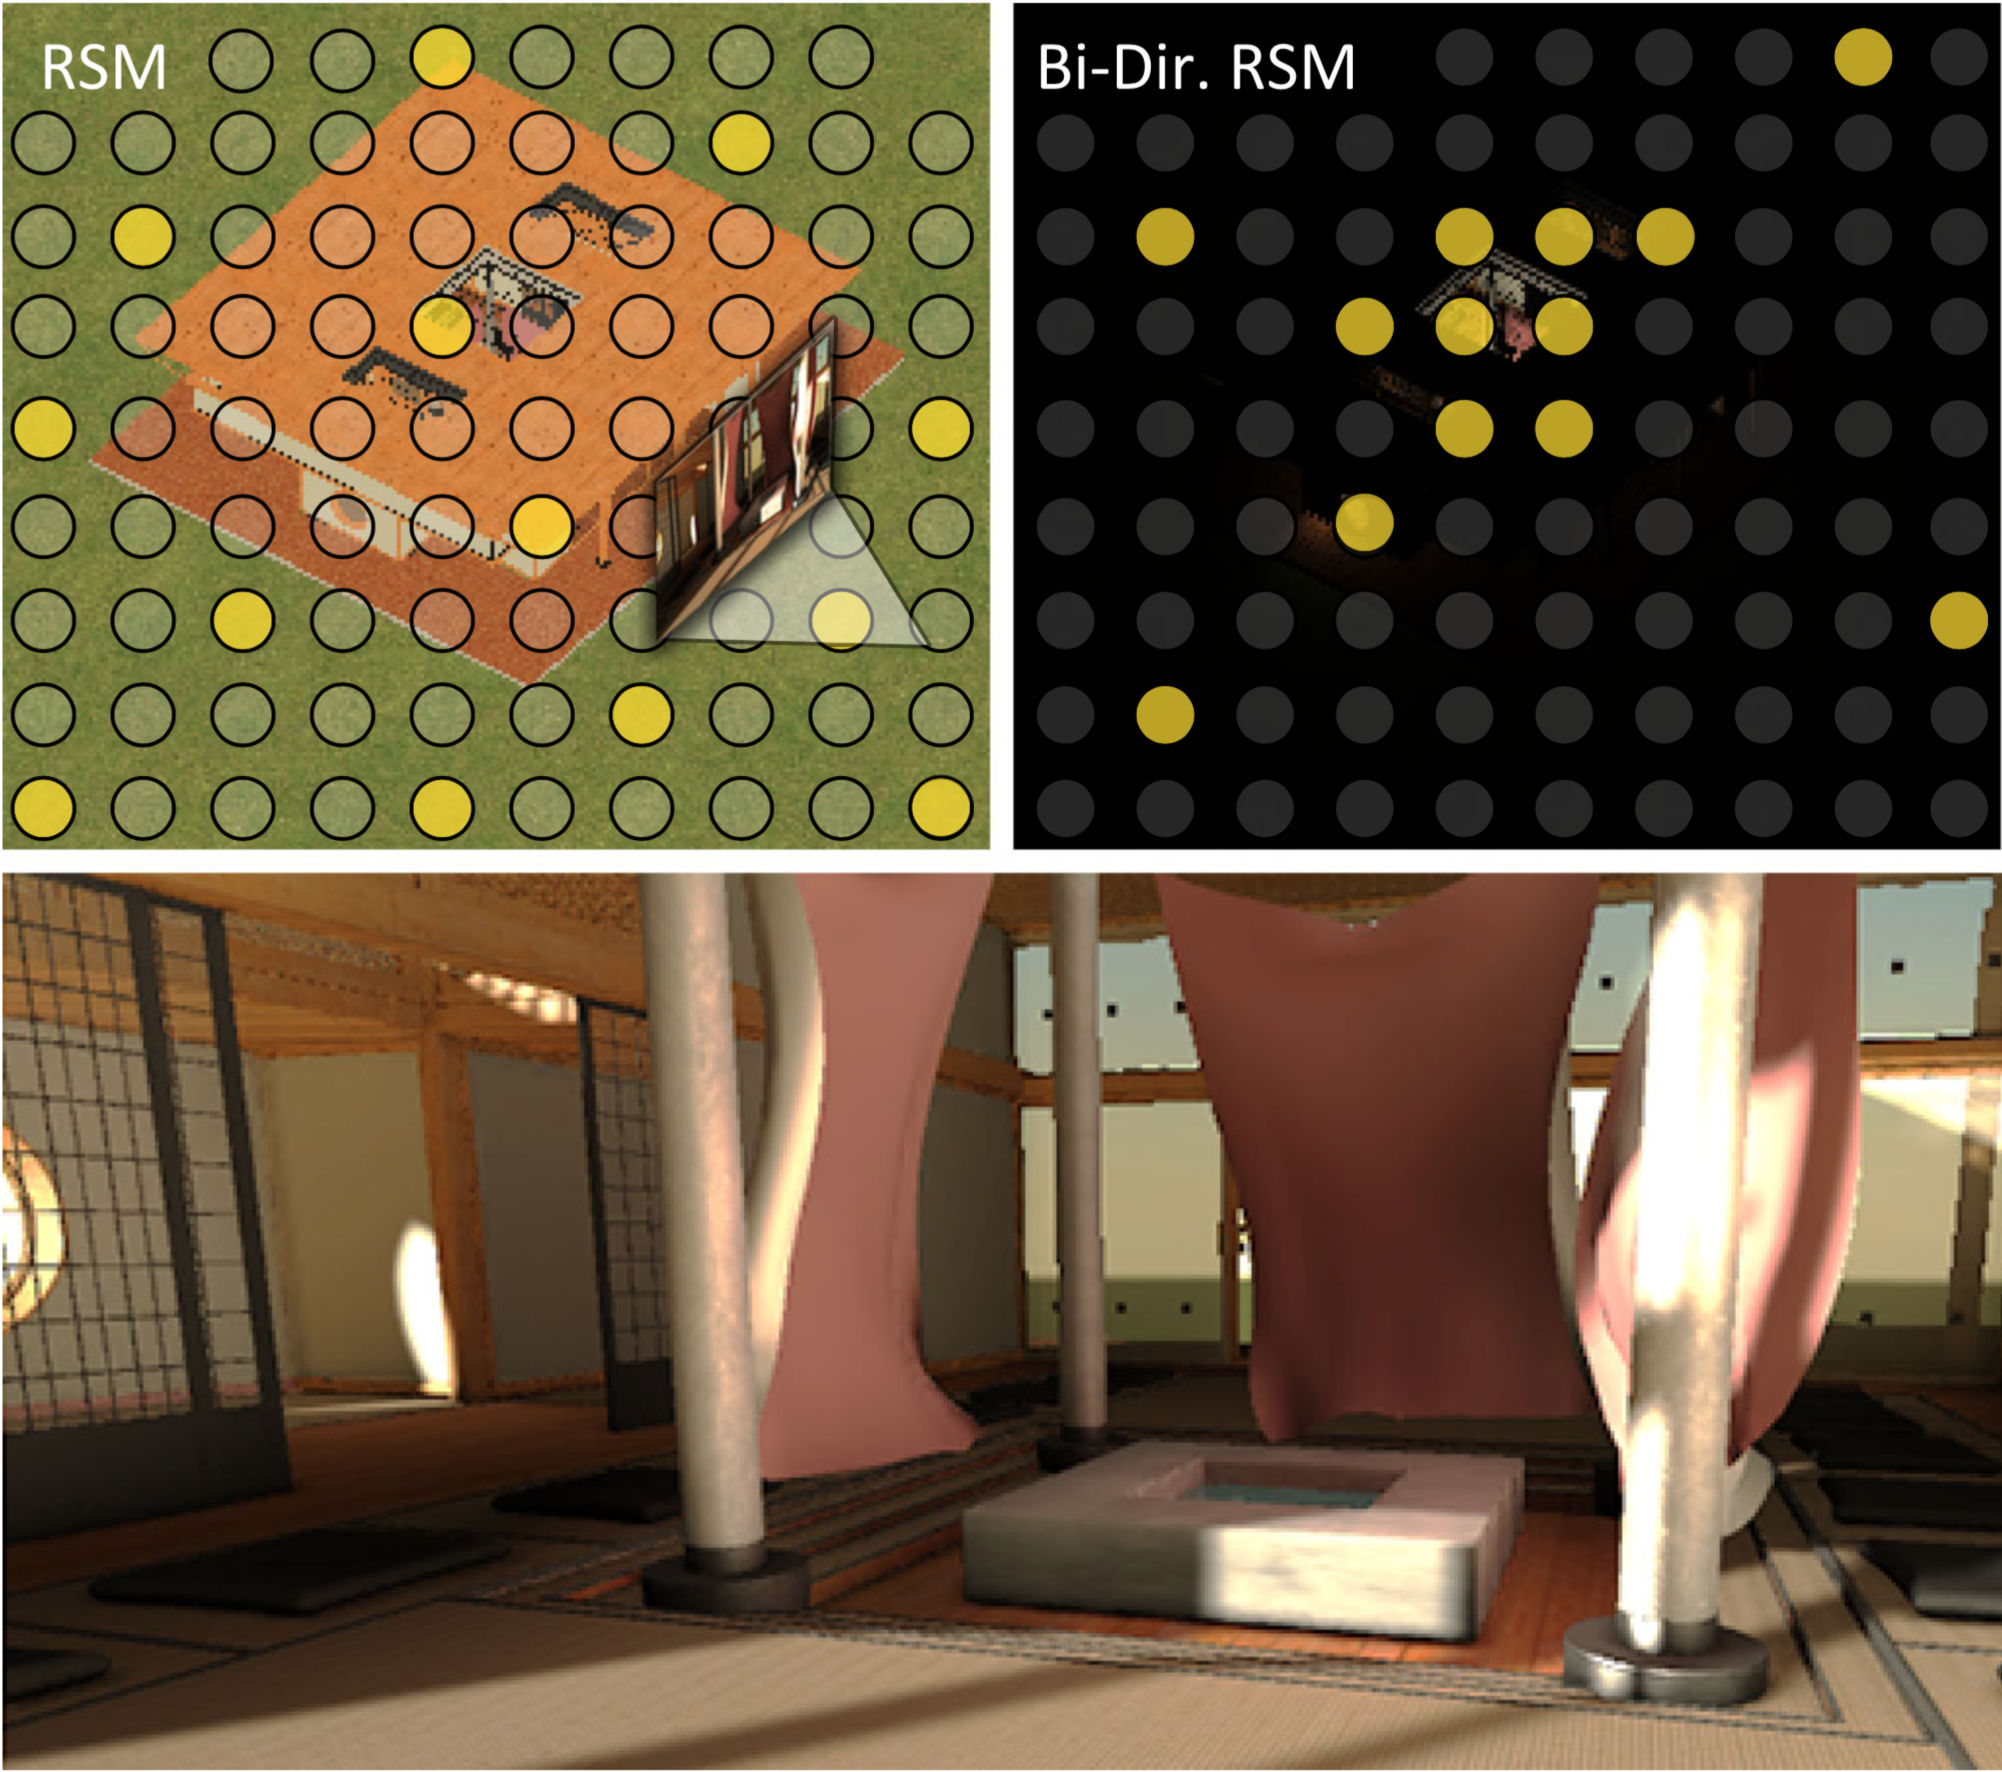
\includegraphics[width=1.\textwidth]{graphics/ir/ir-5-2}
	\end{center}
	\caption{Bidirectional Reflective Shadow Maps sample VPLs according to a distribution that favors VPLs contributing to the current view of the scene. E. g., RSM waste many VPLs on the roof, which have no effect on the final image.}
\end{figure}

They first derive, in parallel, a CDF for each texture column $C_y[i]$ of the BRSM. Second, they compute a single CDF $C_x$ from the sums of all values in each column. Based on these CDFs, they transform a uniform sampling into a sampling that respects the BRSM weights: For a uniform sample $[x,y]^{T}\in[1,\cdots ,width]\times [1,\cdots ,height]$, they first find a column position $i:=C^{-1}_x[x]$, then a row position $j:=C_y[i]^{-1}[y]$, to define the new sample location $[i,j]^{T}$. Figure \ref{f:adaptive-ISMs-2} shows a comparison of our solution against competing methods. Essentially, we transform some random samples into a particular distribution using the inversion method. See section \ref{sec:Transformation-of Random-Variables} in chapter \ref{ch:monte-carlo}.



\subsubsection{Adaptive ISMs}
The reasoning is that occluders will tend to cast smoother indirect shadows on distant receivers which makes it unnecessary to maintain accuracy for distant blockers. On the other hand, small nearby occluders are likely to cast important shadows on nearby view samples and it is crucial to maintain their details.

\begin{figure}\label{f:adaptive-ISMs-4}
	\begin{center}
		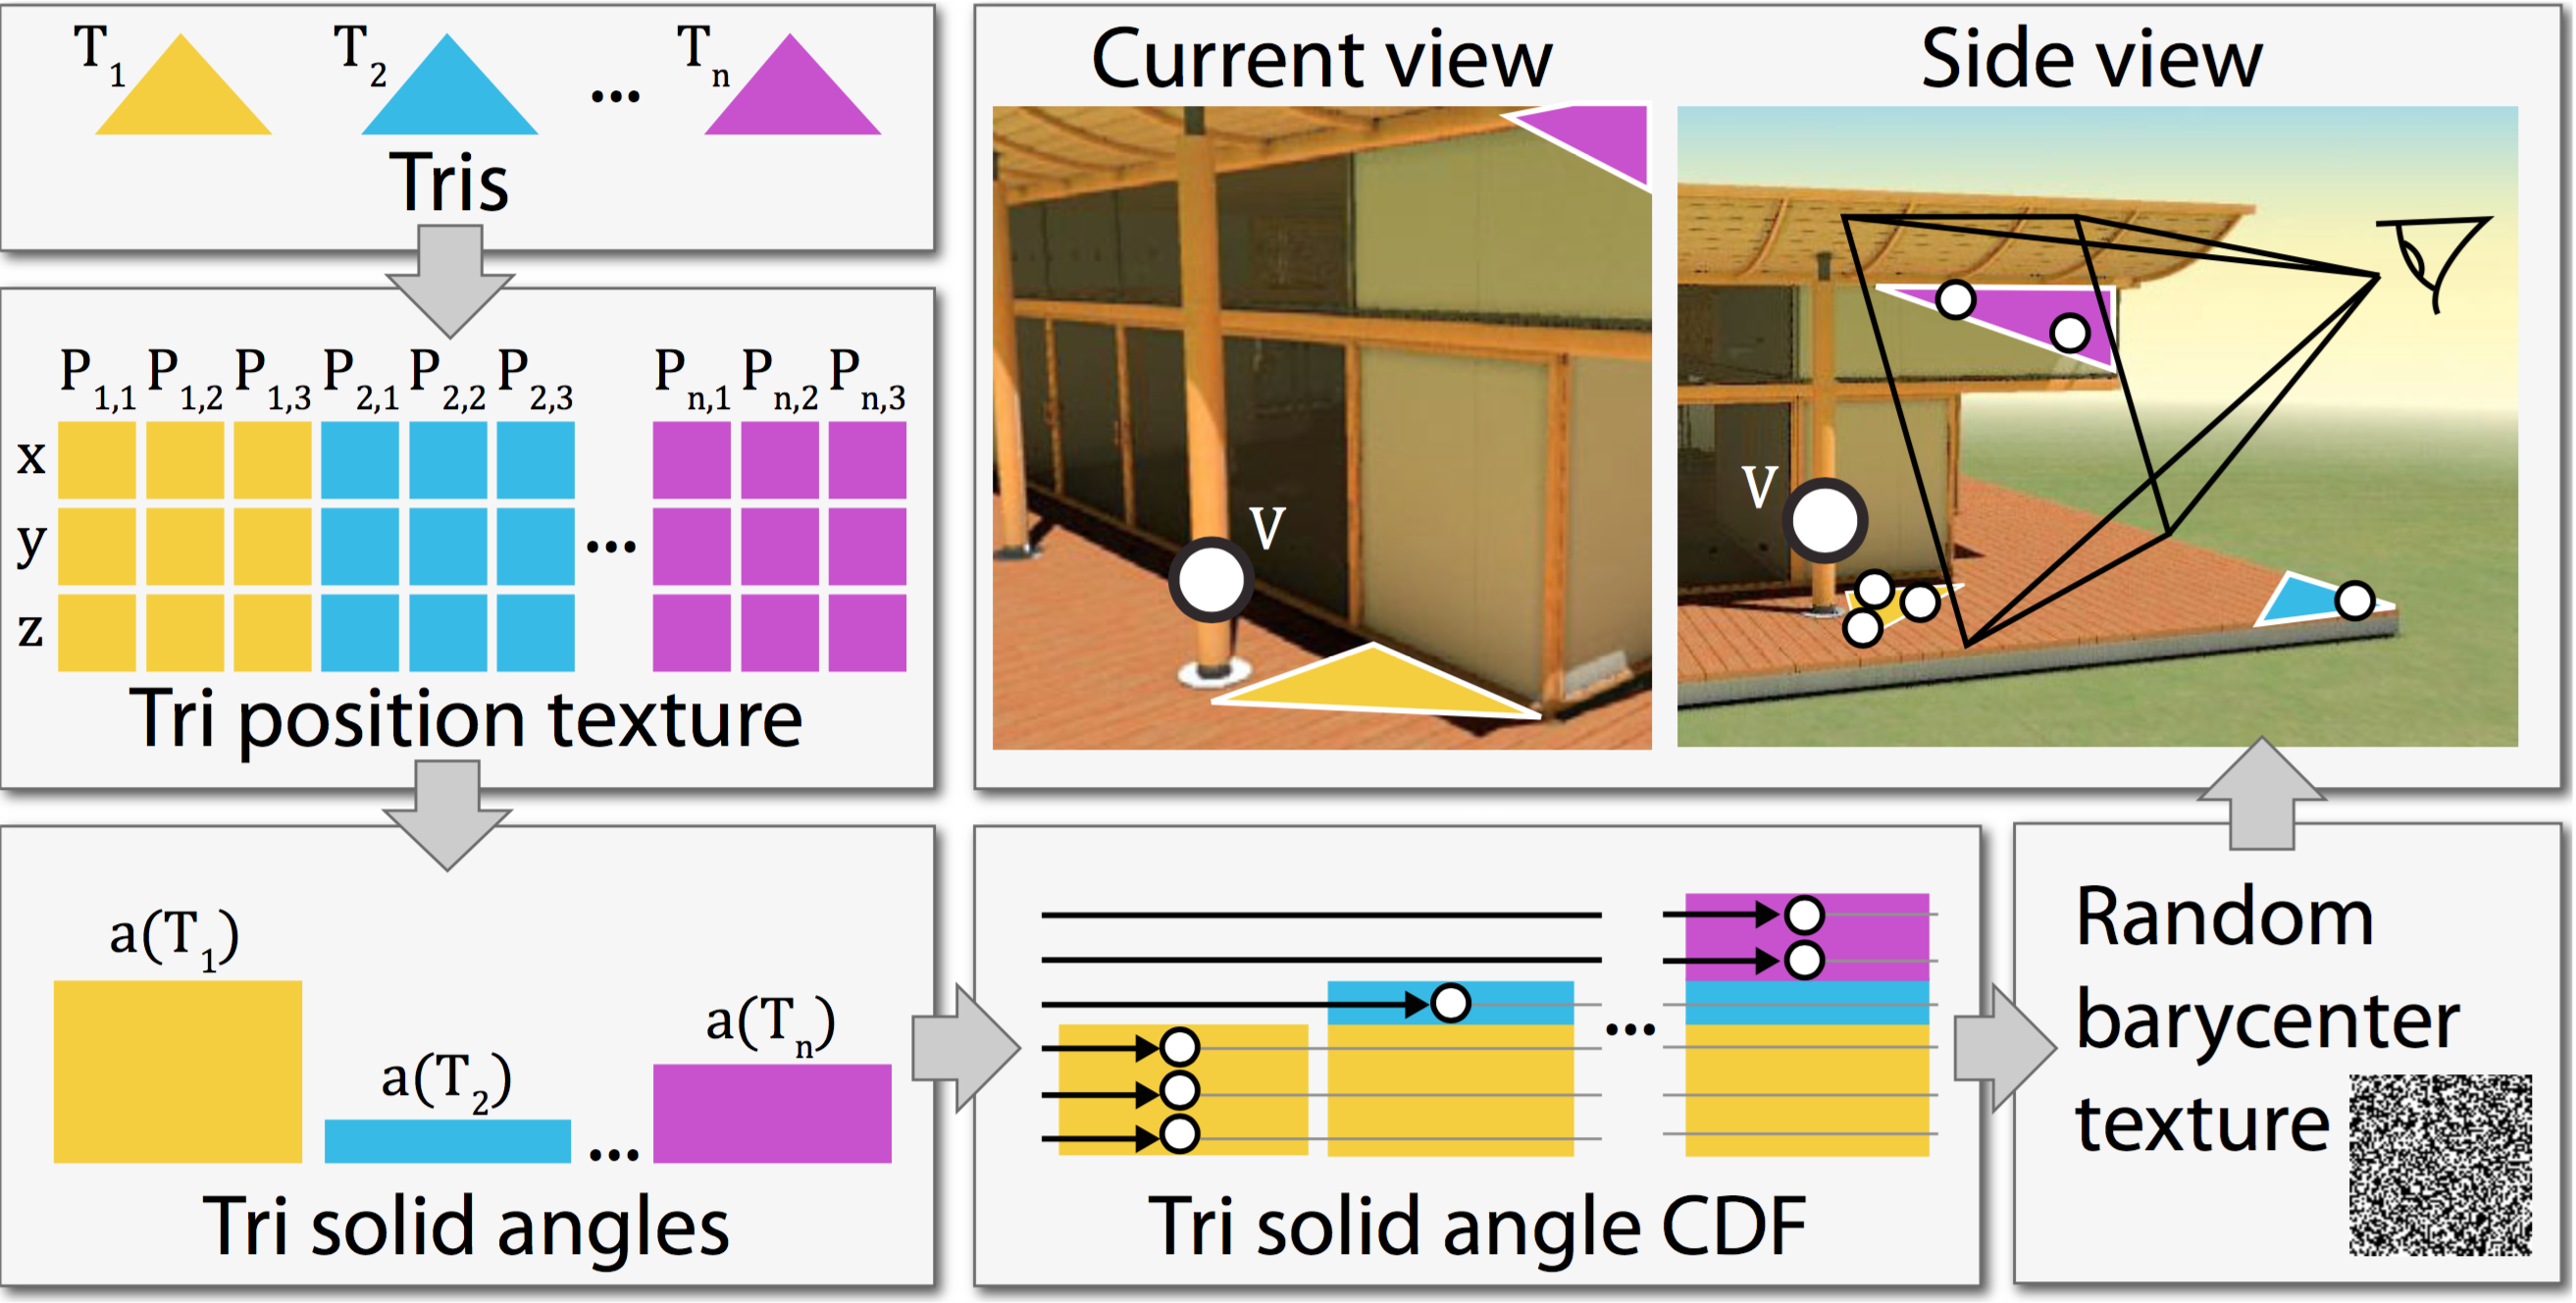
\includegraphics[width=1.\textwidth]{graphics/ir/ir-5-4}
	\end{center}
	\caption{GPU implementation of Adaptive ISMs: For all tris, stored as vertex triples into a texture, their solid angle relative to a given view sample ($V$ , blue circle) is computed. These solid angles are transformed into a cumulative density function (CDF) that is used to sample scene points. Here, the $T_1$ receives more samples than $T_2$ and $T_3$ as it is closer to $V$.}
\end{figure}

They use a $3$-channel \textit{triangle texture} in which it stores the $(x,y,z)$-coords of all vertices of all triangles. Based on this texture, they use a fragment shader to compute a $1$-channel \textit{triangle-importance texture} which stores the solid angle of the $i^{th}$ triangle relative to $V$ in texel $i$. Then they produce, as for the BRSM, a cumulative density function (CDF) stored in a $1$-channel texture of the same size which will guide the point-sampling process of the scene geometry. See figure \ref{f:adaptive-ISMs-4}.




\section{Screen-Space Bias Compensation}
Instant radiosity represents all indirect illumination with VPLs $(\hat{L})$ and replaces all but the first two terms of the Neumann series:

\begin{equation}\label{e:ssbc-1}
	L=\underbrace{L_e}_{\text{emission}}+\underbrace{\mathbf{T}L_e}_{\text{direct illum.}}+\underbrace{\mathbf{T}\hat{L}}_{\text{indirect illum.}}
\end{equation}

One of the main problems of this approach is that lighting from VPLs exhibits singularities in the geometry term $G(x\leftrightarrow y)$ if the VPLs are close to a surface. These singularities cause high intensity speaks that appear in the image as distracting bright splotches. We can remove these artifacts by bounding the geometry term to an arbitrary bound $b: G_b(x\leftrightarrow y)=min(G(x\leftrightarrow y),b)$, resulting in a \textit{bounded transport operator} $\mathbf{T}_b$. This, unfortunately, removes energy from the light transport near edges, corners, and creases, leading to incorrect darkening in these regions.

Jan Novak et al. introduced a method, \textit{screen-space bias compensation}\cite{a:Screen-SpaceBiasCompensationfor}, to improve the quality and correctness of the rendered images by removing bias using a hierarchical screen space approach. They showed that the bias compensation can be formulated as a post-processing step and demonstrate renderings comparable to results from offline algorithms at interactive speed.



\subsection{Efficient Compensation using Residual Transport}
This approach is based on a solid theory obtained from a reformulation of the rendering equation. They express the energy difference between the unbounded and bounded transport operators using a new \textit{residual operator} $\mathbf{T}_r = \mathbf{T}-\mathbf{T}_b$. Then we can reformulate the indirect illumination term in the equation \ref{e:ssbc-1} using the new operators\footnote{
These operators differ only in the geometry term as following:

\begin{equation*}
\begin{aligned}
	\mathbf{T}\hat{L}  &=\sum^{N}_{i=1}f_rGV\hat{L}\\
	\mathbf{T}_b\hat{L}&=\sum^{N}_{i=1}f_r min(G,b)V\hat{L}\\
	\mathbf{T}_r\hat{L}&=\sum^{N}_{i=1}f_r max(G-b,0)V\hat{L}
\end{aligned}
\end{equation*}

where $b$ is the user defined bound. Their results can be see in figure \ref{f:ssbc-1}(a,c and d). 
}:

%\begin{equation*}
%\begin{aligned}
%	\text{Complete LT: }          &L_e+\mathbf{T}L_e+\mathbf{T}\hat{L}&\quad\quad\mathbf{T}\hat{L}&=\sum^{N}_{i=1}f_rGV\hat{L}\\
%	\text{Bounded indirect LT: }  &L_e+\mathbf{T}L_e+\mathbf{T}_b\hat{L}&\mathbf{T}_b\hat{L}&=\sum^{N}_{i=1}f_r min(G,b)V\hat{L}\\
%	\text{Residual indirect LT: } &\mathbf{T}_r\hat{L}&\mathbf{T}_r\hat{L}&=\sum^{N}_{i=1}f_r max(G-b,0)V\hat{L}
%\end{aligned}
%\end{equation*}

\begin{equation*}
	L=L_e+\mathbf{T}L_e+\mathbf{T}_b\hat{L}+\mathbf{T}_r\hat{L}
\end{equation*}

They observe that $\mathbf{T}_r$ also suffers from singularities when being applied to indirect illumination represented by VPLs $(\hat{L})$. To derive a new bias compensation technique, they remove the source of singularities $(\hat{L})$ and replace it by a general reflected illumination $(L-L_e)$ that is not approximated by point light sources. Conceptually, the equation remains the same, the only difference is that $\mathbf{T}_r$ is now integrating reflected light instead of using VPLs (see in figure \ref{f:ssbc-1}(b,c and e)):

\begin{equation*}
	L=L_e+\mathbf{T}L_e+\mathbf{T}_b\hat{L}+\mathbf{T}_r(L-L_e)
\end{equation*}

By recursively expanding this equation we obtain the novel \textit{unbiased} formulation of the rendering equation for IR:

\begin{equation}
	L=L_e+\sum^{\infty}_{i=0}\mathbf{T}^{i}_r(\mathbf{T}L_e+\mathbf{T}_b\hat{L})
\end{equation}

Note $\mathbf{T}_b\hat{L}$ is unbiased. This means that we can compute the unbiased solution as an infinite sum of residual operators that are recursively applied to direct illumination and clamped indirect illumination. The first term of the sum represents the direct and the clamped indirect illumination. Every further summand represents the (clamped) compensation for the clamped contribution of the previous step.

\begin{figure*}\label{f:ssbc-1}
\begin{center}
	\begin{subfigure}[b]{0.195\textwidth}
		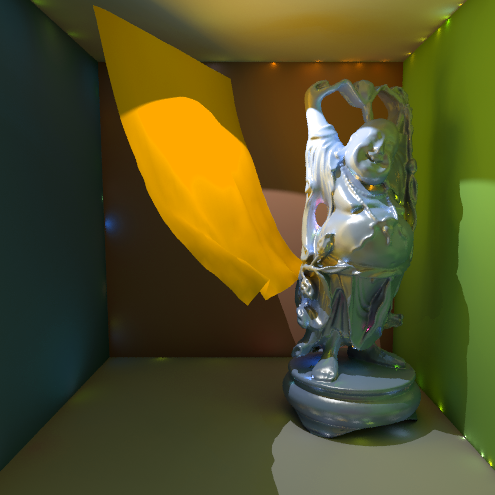
\includegraphics[width=1.0\textwidth]{graphics/ir/ir-7-1}
		\caption{= (c) + (d)}
	\end{subfigure}
	\begin{subfigure}[b]{0.195\textwidth}
		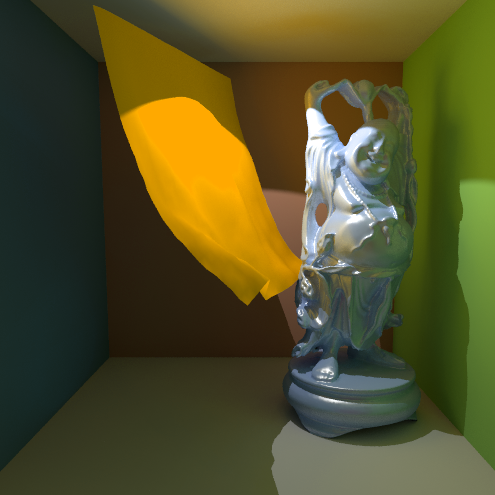
\includegraphics[width=1.0\textwidth]{graphics/ir/ir-7-4}
		\caption{= (c) + (e)}
	\end{subfigure}
	\begin{subfigure}[b]{0.195\textwidth}
		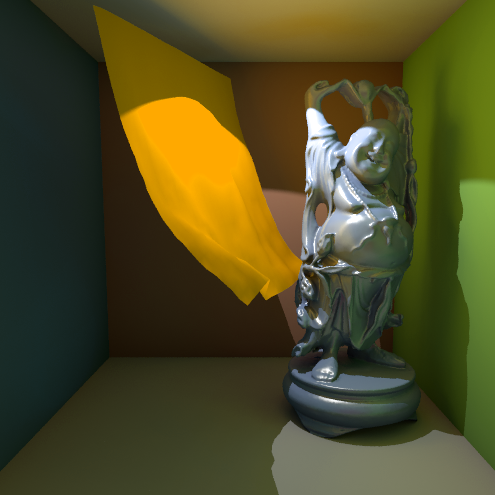
\includegraphics[width=1.0\textwidth]{graphics/ir/ir-7-2}
		\caption{$L_e+\mathbf{T}L_e+\mathbf{T}_b\hat{L}$}
	\end{subfigure}
	\begin{subfigure}[b]{0.195\textwidth}
		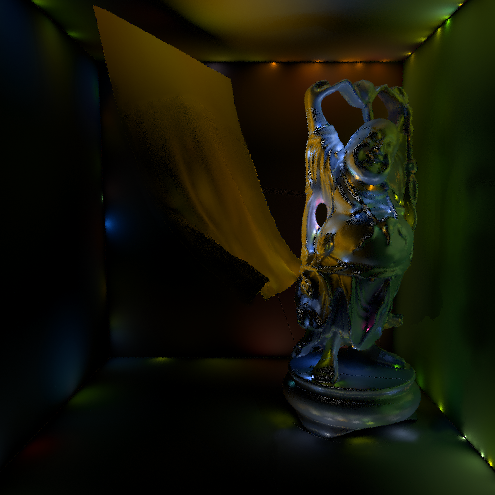
\includegraphics[width=1.0\textwidth]{graphics/ir/ir-7-3}
		\caption{$\mathbf{T}_r\hat{L}$}
	\end{subfigure}
	\begin{subfigure}[b]{0.195\textwidth}
		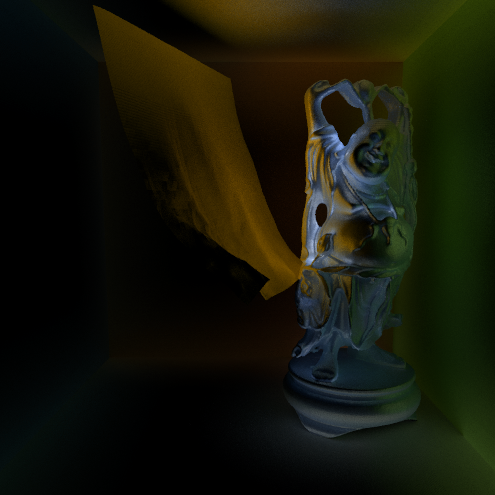
\includegraphics[width=1.0\textwidth]{graphics/ir/ir-7-6}
		\caption{$\mathbf{T}_r(L-L_e)$}
	\end{subfigure}
\end{center}
\caption{Bounded and residual light transport. Note: There are splotches in (a) due to that $\mathbf{T}_r$ also suffers from singularities when being applied to indirect illumination represented by VPLs ($\hat{L}$). But (b) is unbiased because we removed the source of singularities $(\hat{L})$ and replace it by a general reflected illumination $(L-L_e)$ that is not approximated by point light sources.}
\end{figure*}

An important observation is that the energy gain due to the compensation is $(N+1)$-times convolved with the BRDF, and therefore dropping exponentially with increasing $N$. For practical applications, this translates into choosing $N$ such that the visible bias is removed. In their scenes they used $1$ to $3$ iterations, which yielded nearly indistinguishable results from unbiased reference solutions.

Using this reformulation, they derive a new rendering algorithm with bias compensation that consists of two major steps:

\begin{enumerate}
	\item They first compute direct and clamped indirect illumination of each shading point by applying $\mathbf{T}$ to light from primary light sources and $\mathbf{T}_b$ to illumination from VPLs, respectively.
	\item Next, they apply the residual operator iteratively $N$-times to compensate for the clamped contribution.
\end{enumerate}




\subsection{Integration in Screen Space}
Instead of storing shading points over all surfaces, they deal with the bias compensation in screen space which has two major advantages: it applies the residual transport operator as a post-process that operates on the illumination sampled in screen space. Furthermore, it can easily find all surfaces that potentially contribute energy to the compensation, as these have to be nearby in world space, and thus also in screen space.

The transport operators, including $\mathbf{T}_r$, can be formulated as integrals over surfaces. Computing an approximation to $\mathbf{T}_r$ in screen space means that we replace the integral by a sum over a finite number of pixels:

\begin{equation*}
	\mathbf{T}_r\hat{L}\approx\sum^{M}_{i=1}f_r(x\leftarrow y\leftarrow z_i)G_r(y\leftrightarrow z_i)V(y\leftrightarrow z_i)L(y\leftrightarrow z_i)A_i
\end{equation*}

we can obtain these information from a G-buffer of the rendered image, and the surface $A_i$, that the pixel represents in world space, is computed using screen-space derivations.

\begin{figure*}\label{f:ssbc-2}
	\begin{center}
		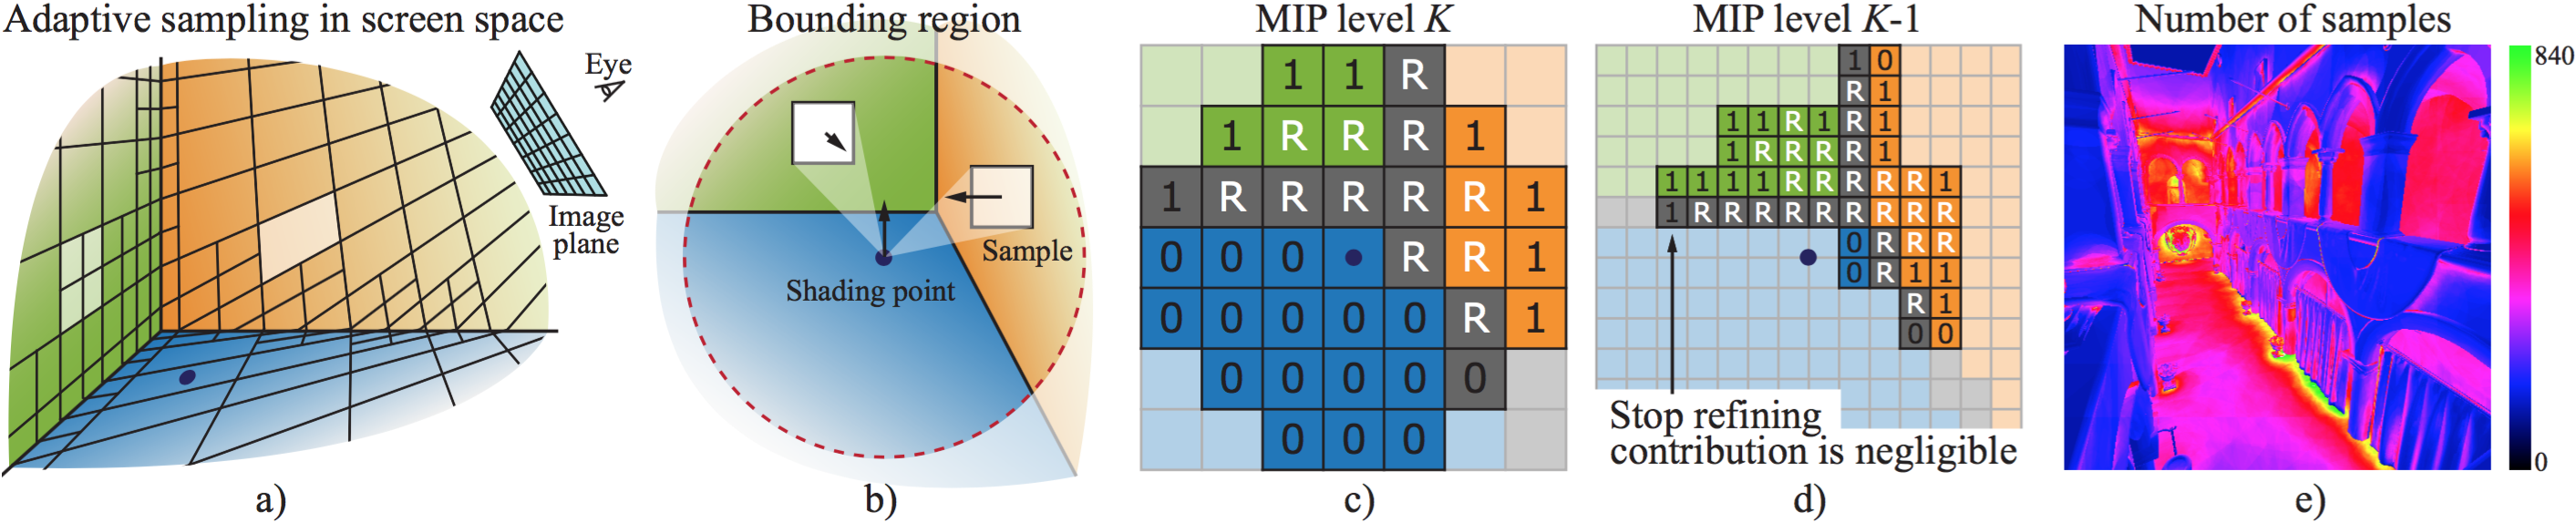
\includegraphics[width=1.\textwidth]{graphics/ir/ir-6-1}
	\end{center}
	\caption{We compute the bias compensation by adaptively applying the residual operator in screen space and projecting individual samples back into world space (a). We first estimate a bounding region (b) that contains all surfaces with possible non-zero contribution, and then, using a hierarchical traversal, evaluate the contribution of individual neighboring samples (c) and (d). Samples spanning discontinuities or subtending a large projected solid angle are refined (R), until their contribution can be estimated accurately ($1$), or drops to zero ($0$). The total number of processed samples for each pixel is for the Crytek Sponza scene shown in (e).}
\end{figure*}

As previously mentioned, only surfaces nearby $y$ contribute to the compensation -- otherwise the geometry term $G_r(y\leftrightarrow z_i)$ becomes zero. We can estimate a spherical bounding region, based on the bound $b$ of $G_b$, in world space that contains surfaces contribution to the compensation as $r=1/\sqrt{b}$ (see figure \ref{f:ssbc-2}(b)), and can be transformed to screen space, e.g. for a perspective projection as $r_s=r/(tan(\delta /2)||x-y||)$, where $\delta$ is the field of view.

Note that $r_s$ depends on the distance from the camera and for closer $y$ the screen space radius becomes bigger spanning more pixels. Since the number of pixels lying inside the bounding bounding region can exceed several thousands. So they derive a hierarchical integration scheme that greatly helps to achieve interactive performance.



\subsection{Hierarchical Integration}
The goal of the hierarchical integration in screen space is to compute the contribution from smooth or more distant (yet still in the bounding region) surfaces using less pixel samples. Figure \ref{f:ssbc-2} demonstrates the general idea of adaptively sampling the integration domain and refining where the information is inaccurate.

For this they compute a mip-map chain for the G-buffer, which contains averaged positions, normals, and material properties, summed pixel areas, and illumination computed from the bounded light transport, i.e. the color of the pixels. They also compute a discontinuity buffer (and a mip-map chain thereof), similarly to Nichols et al.\cite{a:Hierarchicalimage-spaceradiosityforinteractiveglobalillumination}, to avoid integrating over sharp edges and depth discontinuities.

When integrating the surfaces' contributions, for each pixel, they start on the coarsest mip level, and determine whether the computation using this sample is possible to add a contribution. A sample can de divided into three types (see figure \ref{f:ssbc-2}(c)):


\begin{figure}
	\begin{subfigure}[b]{.48\textwidth}
		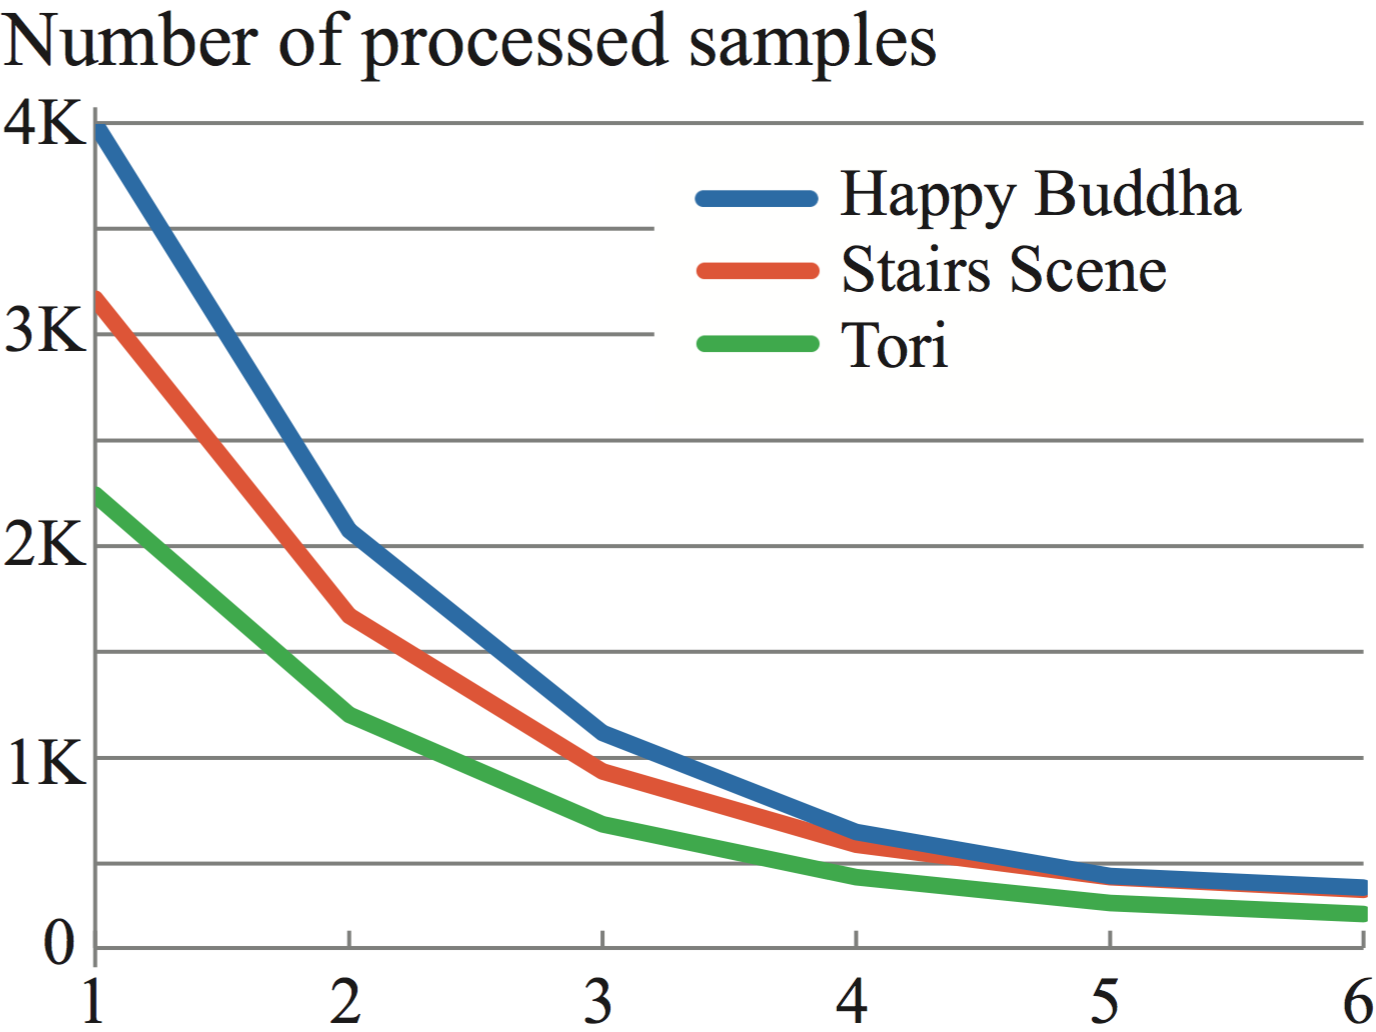
\includegraphics[width=1.\textwidth]{graphics/ir/ir-7-7}
		\caption{No. of levels in the hierarchy}
	\end{subfigure}
	\begin{subfigure}[b]{.48\textwidth}
		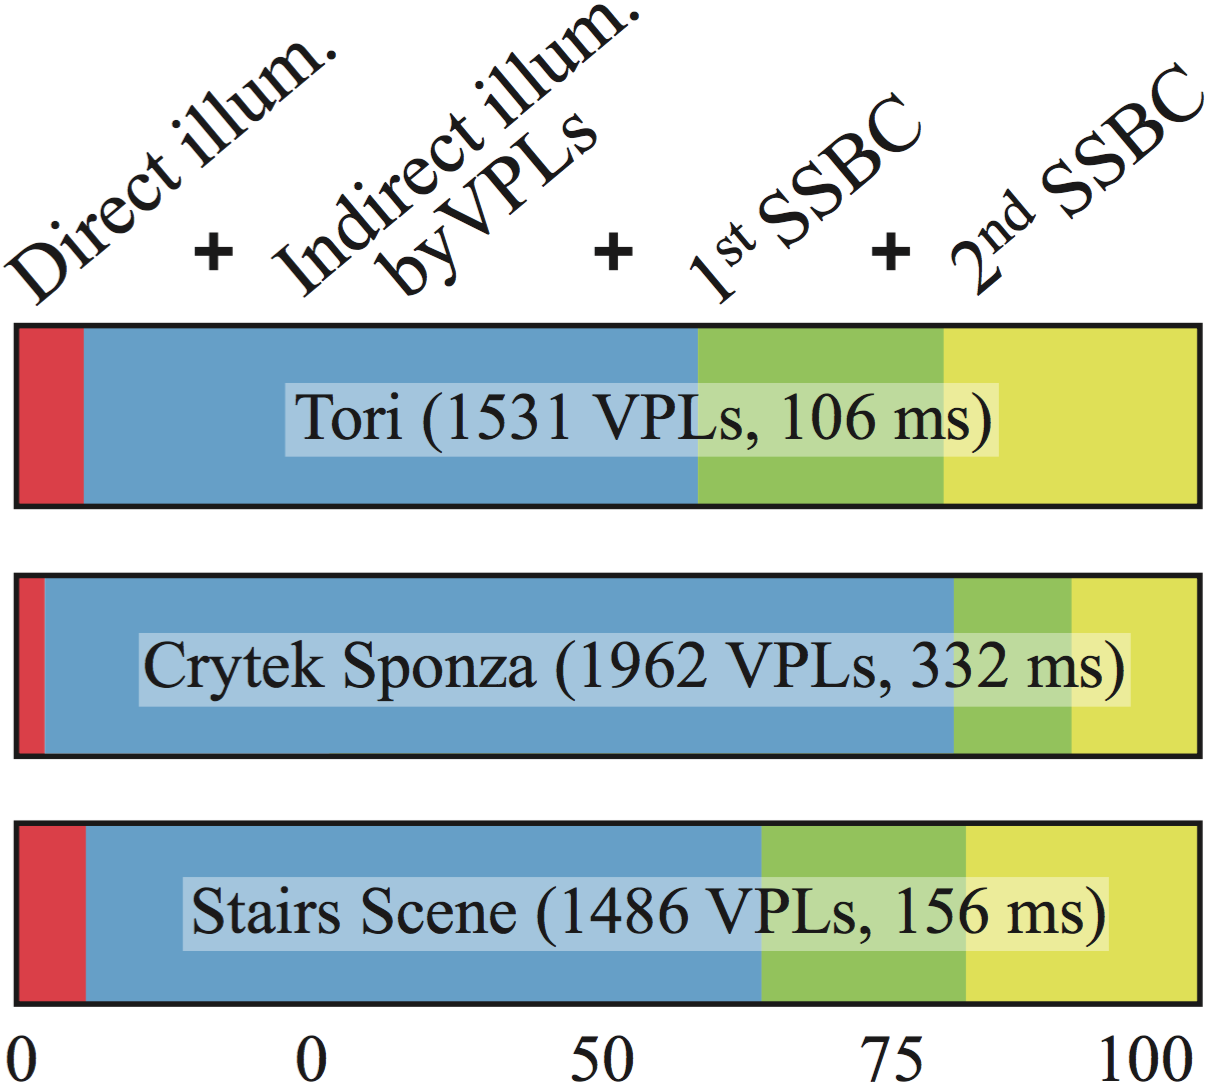
\includegraphics[width=1.\textwidth]{graphics/ir/ir-7-8}
		\caption{Relative execution time}
	\end{subfigure}
	\caption{a) The average number of samples per pixel used for bias compensation is highly dependent on the number of mip levels used for the hierarchical G-buffer. b) Relative time spent on the different tasks: the cost of 2 compensation steps is moderate compared to that of computing illumination from VPLs. The number of VPLs and the total rendering time is given in parentheses.}
\end{figure}




\begin{itemize}
	\item $1$: non-zero contribution.
	\item $0$: zero contribution.
	\item $R$: must be refined.
\end{itemize}

In order to avoid spatial and temporal artifaces in dynamic scenes, we have to refine and proceed to the next mip level if (see figure \ref{f:ssbc-2}(d)):

\begin{enumerate}
	\item G-term too high: 
	\item Discontinuity: 
\end{enumerate}
 
If at least one of the criteria is met, we omit the sample and refine by recursively integrating over the four corresponding pixels at the next finer level. The second criterion can cause a lot of refinement in areas with negligible contribution, e.g. distant surfaces. Therefore, we only refine at discontinuities when the projected solid angle is higher than a user specified threshold ($\approx 0.04)$. This significantly improves the performance without introducing noticeable artifacts, as it is only effective for samples with low contribution.
 
 


\section{Many-Light Methods}


\subsection{Lightcups}
\subsection{Matrix Row-Column Sampling}
\subsection{LightSlice}
\subsection{Efficient Shadows for Many Lights}
\subsection{Practical Clustered Shading}
\subsection{Shadows for Many Light}


Their rendering cost is sublinear in the number of point lights, thus enabling rendering from an extremely large number of light sources.


Many-light approaches are a variant of IR that abstracts from the way VPLs are produced.



The lightcuts method [Walter et al. 2005] groups a large number of light samples (VPLs representing the indirect illumination) into a hierarchy to speed up rendering. Visibility between a surface point and a node in the hierarchy (a collection of VPLs) is approximated with a single shadow ray. However, the algorithm bounds the resulting error, such that no perceptible artifacts appear. 













15| Efficient Shadows for Many Lights




















